% Management Science template requested by the author:
% https://www.overleaf.com/latex/templates/template-for-management-science-journal/bjpqpdqhbshy
\documentclass[mnsc,blindrev]{informs3}

\OneAndAHalfSpacedXI

\usepackage{mathtools}
\usepackage{booktabs,tabularx,array}
\usepackage{enumitem}
\usepackage{tikz}
\usetikzlibrary{arrows.meta,positioning,calc}
\usepackage{natbib}
\bibpunct[, ]{(}{)}{,}{a}{}{,}
\def\bibfont{\small}
\def\bibsep{\smallskipamount}
\def\bibhang{24pt}
\def\newblock{\ }
\def\BIBand{and}
\usepackage{xcolor}
\usepackage[colorlinks=true,allcolors=blue!45!black]{hyperref}

\EquationsNumberedThrough
\TheoremsNumberedThrough
\ECRepeatTheorems

\newcommand{\E}{\mathbb E}
\newcommand{\calE}{\mathcal E}
\newcommand{\R}{\mathbb R}
\newcommand{\ind}{\mathbf 1}
\newcommand{\ph}{\phi}
\newcommand{\DataRequired}{\textsc{Data Required}}
\newcolumntype{L}[1]{>{\raggedright\arraybackslash}p{#1}}

\MANUSCRIPTNO{}
\RUNAUTHOR{Anonymous Authors}
\RUNTITLE{Announced Rescue Pricing and the Screening History of Supply}
\TITLE{Announced Rescue Pricing: Strategic Waiting, Screening History,
and Market Thickness}
\ARTICLEAUTHORS{}

\begin{document}

\ABSTRACT{A platform that announces a higher payment for an unfilled request
improves its chance of rescue but also gives current suppliers a reason to
wait.  We study this trade-off when the expected thickness of the incumbent
driver pool is public, its realization is latent, and universal rejection
both triggers continuation and screens the remaining supply.  A private-value
rider decides whether to post and, after failure, whether to abandon, repeat,
or activate rescue; private-cost incumbents decide whether to accept the
initial payment or preserve a discounted option to wait.  Within an anonymous
symmetric cutoff-WPBE class, we characterize equilibrium with incumbent
survival and fresh driver entry.  In the uniform no-entry core, every menu has
a unique cutoff and the two-payment design reduces to a one-dimensional
optimization.  The optimal rescue menu strictly improves completion above an
endogenous patience threshold.  Its completion gain relative to the optimal
flat payment is continuous in market thickness, vanishes in both very thin
and very thick markets, and therefore attains a positive maximum at a finite
thickness; uniqueness of that maximizer is not asserted.  With both surviving
incumbents and fresh entrants, a small rescue strictly beats optimized flat
pricing whenever at least one optimal flat price leaves the highest rider type
strictly willing to use rescue.  Holding either continuation headcount or
price-marginal capacity fixed, a larger incumbent share strictly intensifies
first-order strategic waiting within the active local-rescue region, while
its completion effect can reverse with incumbent
patience.  We also provide a pre-specified model-to-data mapping for a
request-level structural calibration; quantitative estimates are deliberately
withheld until the announcement, exposure, and entry measurements required by
the model are available.}

\KEYWORDS{dynamic pricing, rescue payments, strategic waiting, market
thickness, screening, Poisson games}

\maketitle

\section{Introduction}
\label{sec:introduction}

Recent reporting makes the operational problem concrete.  In January 2026,
DoorDash warned that severe-weather demand could outstrip available couriers,
producing long waits and cancelled orders; its stated response included a
temporary fee passed through to active couriers as Peak Pay
\citep{DoorDash2026}.  Reuters documented a sharper rejection mechanism in
Kenya: some ride-hailing drivers asked riders to pay more than the app price
and cancelled the request when the rider declined, sending the rider back to
search for another driver \citep{Okoth2024}.  Continuation supply can change
as well.  Reuters reported that JD.com doubled its three-month recruitment
target for full-time delivery riders from 50,000 to 100,000
\citep{Reuters2025JD}.  These episodes establish the separate forces of
scarcity, rejection, higher compensation, rematching, and fresh entry; they do
not establish the exact same-request contract studied here.  We ask whether
committing ex ante to a higher payment after universal rejection rescues a
request or instead teaches incumbents to wait for the next offer.

Many service requests are initially unattractive to available suppliers but
become urgent after a failed response window.  A platform can address this
problem by announcing an initial payment and a higher, failure-contingent
rescue payment.  Announcement makes the policy credible, but it also changes
the first response: a supplier may reject today in order to preserve the
option of receiving more tomorrow.  The platform must therefore design the
rescue schedule and the induced waiting equilibrium jointly.

This tension is especially sharp when the platform observes an expected
market state but not the realized local supply attached to a particular
request.  Universal rejection is then both an operational event and an
informational event.  It triggers the second response window and reveals that
every incumbent who was willing to accept the initial payment is absent from
the continuation pool.  Incumbents who remain are selected by their earlier
rejection, whereas drivers who enter later have not been screened.  The value
of future supply consequently depends on its screening history, not only on
its expected quantity.

We study a two-period request in which a platform commits to payments
$(p_1,p_2)$ with $p_2\ge p_1$.  A private-value rider first decides whether to
post.  Private-cost incumbent drivers then simultaneously accept $p_1$ or
wait.  After universal rejection, the rider can abandon, repeat $p_1$, or
activate $p_2$.  Incumbents may survive to the second window and a fresh pool
may enter.  The expected incumbent thickness is public, while realized local
supply and rival costs remain latent.  Drivers who wait discount their
terminal payoff, and accepting drivers compete for assignment.

The analysis follows a policy--response--optimization sequence.  We first fix
the announced menu and characterize weak perfect Bayesian equilibrium within
the anonymous symmetric pure-cutoff class.  We then optimize the menu subject
to that equilibrium response.  Universal rejection generates a tractable
failure posterior: incumbents remaining above the first-period cutoff are a
screened population, while fresh entrants retain the original cost
distribution.  The equilibrium characterization allows arbitrary incumbent
survival and fresh entry and makes the rider's abandon--repeat--rescue choice
part of the drivers' continuation payoff.

The globally solvable core sets fresh entry to zero while retaining incumbent
survival.  In the uniform model, every announced menu has a unique equilibrium
cutoff.  For a fixed $p_1$, the optimal rescue problem separates into
reject-all, tangent-rescue, and repeat-only regimes.  This reduces joint design
of $p_1$ and $p_2$ to a continuous one-dimensional problem and proves policy
attainment.  Above an endogenous rider-patience threshold, the optimized
rescue menu strictly improves completion relative to the optimized flat
payment.  Positive incumbent survival makes $\beta\ge1/2$ a simple sufficient
condition at every finite thickness.

We next return to the general continuation pool.  When $\alpha<1$ and
$\gamma>0$, the second window contains both screened surviving incumbents and
unscreened new entrants.  A local theorem shows when a small announced rescue
increase improves completion after accounting for both sources of supply.  If
at least one optimized flat price satisfies this activity condition, the same
perturbation proves strict policy-class dominance over optimized flat pricing,
without requiring the flat optimizer to be unique.  A separate composition
theorem holds either the expected continuation headcount or the local
price-marginal capacity fixed.  Replacing entrants with screened incumbents
strictly strengthens first-period acceptance erosion; its effect on the local
completion gain has no unconditional sign and can reverse with $\delta$.

Market thickness determines where rescue design matters.  Let $M_R^*(m)$ and
$M_F^*(m)$ denote the optimized completion probabilities under rescue and flat
pricing at the same thickness.  Their difference $V(m)$ is continuous,
vanishes in very thin and very thick markets, and is strictly positive at some
finite thickness.  Hence a finite intermediate market maximizes the rescue
gain.  This existence result does not imply that $V(m)$ is strictly
single-peaked or that the maximizing thickness is unique.

The paper also specifies a request-level empirical implementation.  The data
must record the announced menu, the initial exposure set, universal rejection,
rider continuation, incumbent survival, fresh entry, and terminal completion.
Those inputs are not present in the current repository.  We therefore provide
a pre-specified measurement map, calibration criterion, validation design, and
counterfactual pipeline, with every empirical result explicitly marked
\DataRequired.  Assumed-parameter computations remain theoretical numerical
illustrations rather than empirical estimates.

This paper makes three contributions.  First, it characterizes the
cutoff-WPBE created by an announced same-request rescue menu, latent local
competition, and a private rider continuation decision.  Second, it solves
the global no-entry design problem and establishes how patience and market
thickness govern the completion gain from rescue pricing.  Third, it
separates screened surviving incumbents from unscreened fresh entrants,
establishes conditional optimized-flat dominance in the mixed-supply model,
and proves that composition matters even when continuation headcount or
price-marginal capacity is held fixed.  The contribution is the equilibrium and
completion-design analysis generated by this joint structure, not the
procurement-clock architecture, strategic waiting, entry, or market thickness
in isolation.

The remainder of the paper reviews the closest literatures, states the
empirical measurement requirements, develops the model and equilibrium,
solves the design problem, studies thickness and supply composition, and lays
out the calibration and policy-counterfactual procedure.  Proofs and numerical
verification details appear in the appendices.

\section{Literature Review}
\label{sec:literature}

\paragraph{Procurement clocks and strategic timing.}
\citet{LiKuo2013} optimize a finite discrete Dutch auction that advances after
universal nonacceptance, permits a Poisson number of bidders, and randomly
selects among simultaneous acceptors.  Reversing the transfer direction gives
the low-to-high procurement skeleton of an announced rescue menu.
\citet{BuchananEtAl2016} derive symmetric Bayesian bidding when realized group
size is hidden and nonacceptance changes beliefs along a multi-unit Dutch
clock.  \citet{CarareRothkopf2005} study slow Dutch auctions with waiting
costs, and \citet{Shneyerov2014} optimizes a dynamic clock when market sides
discount at different rates.  These papers establish the importance of
strategic timing, population uncertainty, and learning from nonacceptance.
Our posted-payment environment instead embeds the clock in a private rider's
continuation problem and evaluates unconditional request completion.

Search mechanisms provide a second foundation for the continuation pool.
\citet{McAfeeMcMillan1988} study dynamic mechanisms that acquire additional
participants over time.  \citet{CremerEtAl2007} formulate optimal search
auctions in which previously contacted bidders are incumbents and later
search brings new entrants; a rejected incumbent can therefore remain in a
subsequent allocation with a newly solicited bidder.  These papers establish
retained incumbency and fresh entry before strategic delay is added.

\citet{LeeLi2023} is especially close to the survival-and-entry extension.
Their seller commits to a reserve-price and sampling schedule; long-lived
incumbent bidders can bid or wait, new bidders enter later, and earlier
screening truncates the values of the incumbent pool while new bidders retain
the original distribution.  Under the procurement dual, this is the same
screened-incumbent versus unscreened-entrant distinction that appears here.
Their analysis establishes announced price paths, strategic waiting, and the
mixed composition of future supply in a search-auction environment.  Our
setting instead uses an anonymous posted-payment allocation with latent Poisson
competition, a rider who chooses among abandon, repeat, and rescue, and
completion comparisons between optimized rescue and flat policies.

\paragraph{Announced dynamic pricing and forward-looking agents.}
\citet{AvivPazgal2008} solve announced markdown design by fixing a price path,
deriving a forward-looking consumer threshold, and then optimizing the path.
\citet{CorreaEtAl2016} study contingent pricing with strategic consumers.
These papers supply the methodological policy--response--optimization order,
but their consumers wait for a lower price and face stockout.  Here suppliers
wait for a higher payment and face assignment competition.  In two-sided
markets, \citet{ChenHu2020} study Poisson arrivals with strategic waiting, and
\citet{HuHuZhu2022} obtain both high--low and low--high surge paths from rider
and driver temporal responses.  The present model isolates a single request,
an ex ante failure-contingent menu, and the posterior created by universal
rejection.

\paragraph{Platform bonuses, dispatch, and strategic rejection.}
\citet{WuEtAl2022} optimize multistage order-specific bonuses in meal delivery
using an acceptance model driven by the current bonus.  Their fixed-later-bonus
ablation finds no detectable anticipation before that bonus, although the
future path is not described as disclosed and committed.  This evidence is an
external-validity challenge for the strategic channel studied here and makes
announcement timing an empirical requirement.  \citet{SiggEtAl2025} model
workers who reject a delivery request so that it is reoffered at a higher
payment.  Broadcast, supplier-menu, and notification models also study
contention and a second attempt after no response, but vary outreach,
assignment, or demand batching rather than solve the same-request announced
payment game \citep{SunEtAl2020,HornerEtAl2021,AusseilEtAl2022,
FengEtAl2023,QinEtAl2025}.

\paragraph{Latent supply, strategic availability, and market thickness.}
\citet{Chen2012} derives private-cost sellers' willingness to wait for higher
buyer offers when the seller count is fixed and public and the buyer does not
precommit.  \citet{BaiEtAl2023} let a platform announce a supply-contingent
price and compensation rule when true supply is random and providers can hide
availability.  Strategic rejection, relocation, and acceptance are likewise
established in ride-hailing and service-platform models
\citep{GudaSubramanian2019,GargNazerzadeh2022,AfecheEtAl2023,
FengWang2023,MeskarEtAl2023}.  Poisson population uncertainty determines our
assignment and failure posteriors, but Poisson supply and market thickness are
tools rather than standalone contributions.

Market thickness itself has direct theoretical and operational precedents.
\citet{LoertscherMuirTaylor2022} balance gains from accumulating traders
against delay in a dynamic bilateral-trade mechanism.  Using online food-
delivery operations, \citet{ZhaoPapierTeo2024} show how processing time changes
the thickness available for matching.  Together they establish the broader
economics of intermediate and optimally chosen market thickness.  Our object
holds $m$ fixed and compares two payment-policy classes:
$V(m)$ is the completion advantage of optimal rescue pricing over optimal flat
pricing in that same environment.

Empirical work has also structurally quantified matching and participant
responses in ride-hailing.  For example, \citet{ZhangEtAl2026} estimate driver
acceptance and relocation together with rider choice in a centralized matching
system.  The empirical implementation here consequently requires variation
that disciplines announced same-request rescue, screening history, and rider
continuation in addition to driver acceptance and market density.

Against these literatures, we characterize the
cutoff-WPBE and completion-design problem created jointly by an ex ante
same-request posted-payment menu, latent realized competition, a private
rider's post-failure continuation, and a continuation pool containing screened
incumbents and potentially unscreened entrants.  The global design and
thickness theorems are proved for the stated uniform no-entry core; the entry
extension is local and its global policy comparisons remain numerical.

\section{Institutional Setting and Empirical Requirements (Protocol Only)}
\label{sec:data}

This section records the empirical contract that must be satisfied before the
model can be called calibrated.  The current repository contains no request-
level data, data dictionary, announcement protocol, or exposure table.
Accordingly, every empirical entry below is marked \DataRequired, and no
parameter value in the paper is described as an estimate.

\subsection{Operational setting and policy timing}

An empirical implementation requires a platform on which one request is shown
to a well-defined incumbent response set, both $p_1$ and the failure-contingent
$p_2$ are credibly disclosed before the first response, and a second response
window follows universal rejection.  The logs must distinguish three events:
an incumbent who remains eligible, a newly eligible entrant, and a driver who
was never exposed.  They must also show whether the rider abandons, repeats
$p_1$, or activates $p_2$.  A no-acceptance record without the corresponding
exposure set cannot distinguish universal rejection from zero supply.

The theoretical transfer is paid by the rider to the selected driver and the
objective is completion.  If the empirical payment is a platform-funded bonus,
a fare component, or a bundled transfer, the incidence must be documented and
the mapping treated as a reduced-form calibration rather than an exact
institutional identity.  Profit, subsidy expenditure, and welfare require
additional primitives and are not implied by a completion-maximizing model.

\subsection{Data construction and measurement map}

The empirical unit is a request--response-window record linked to driver-level
exposures and rider continuation events.  Table~\ref{tab:measurement} is the
minimum measurement map.  Raw or restricted observations must remain outside
Git; only schemas, aggregate outputs, and reproducible code belong in the
repository.

\begin{table}
\TABLE
{Model-to-data measurement map (design only; no estimates).\label{tab:measurement}}
{\begin{tabularx}{\textwidth}{L{16mm}L{42mm}XL{25mm}}
\toprule
Object & Economic meaning & Required empirical counterpart & Status\\
\midrule
$p_1$ & Initial payment & Amount displayed to each side before the first response & \DataRequired\\
$p_2$ & Committed rescue payment & Amount and disclosure timestamp preceding first-round decisions & \DataRequired\\
$m$ & Public expected incumbent thickness & Logged supply forecast or pre-decision market-state proxy & \DataRequired\\
$N^I$ & Latent realized incumbent count & Initial eligible/exposed roster, used through a measurement model & \DataRequired\\
$\alpha$ & Incumbent survival & Same driver remains eligible after universal rejection & \DataRequired\\
$\gamma m$ & Fresh supply intensity & Newly eligible second-window drivers not in the incumbent roster & \DataRequired\\
$\beta$ & Rider continuation factor & Posting and abandon/repeat/rescue choices across delay and payment variation & \DataRequired\\
$\delta$ & Incumbent waiting factor & Same-driver decisions across windows and waiting-time variation & \DataRequired\\
$F,G$ & Cost and value distributions & Choice variation with exposure denominators and exogenous payments & \DataRequired\\
\bottomrule
\end{tabularx}}
{Expected thickness $m$ is not an observed realization of $N^I$.  Each
parameter will be classified as measured, estimated, calibrated, or fixed for
sensitivity before empirical results are reported.}
\end{table}

The sample-construction table will report the data source, markets, dates,
randomization or policy arms, original request count, exclusions, missingness,
censoring, and final linked sample.  Descriptive evidence will separately show
first-window acceptance, universal rejection, rider continuation, rescue
activation, terminal acceptance, and completion across thickness cells.

\subsection{Identification gates}

The announced-rescue channel is empirically identified only if $p_2$ was
known and credible before incumbents chose whether to accept $p_1$.  Static
price variation can discipline current-payment acceptance and the flat
benchmark, but cannot by itself identify anticipatory waiting.  Endogenous
menu assignment requires an instrument or a transparent selection model.
Likewise, $\alpha$ and $\gamma$ cannot be separated without persistent driver
identifiers and response-window eligibility records.

Until these gates are met, the empirical contribution is a pre-specified
design rather than a result.  Section~\ref{sec:calibration} states the
calibration criterion, validation moments, uncertainty procedure, and
counterfactuals that will be populated when the required inputs become
available.

\section{Model}
\label{sec:model}

\subsection{Primitives and policy}

Table~\ref{tab:primitives} defines the primitives once.  The analytical
results below impose $F(c)=c$ and $G(v)=v$ on $[0,1]$; the empirical design
allows parametric or semiparametric alternatives and must label that change
explicitly.

\begin{table}
\TABLE
{Model primitives and empirical counterparts.\label{tab:primitives}}
{\begin{tabularx}{\textwidth}{L{15mm}L{22mm}XL{39mm}}
\toprule
Symbol & Domain & Economic meaning & Empirical counterpart\\
\midrule
$p_1,p_2$ & $0\le p_1\le p_2\le1$ & Initial and committed rescue payments & Displayed menu and timestamps\\
$m$ & $(0,\infty)$ & Public expected incumbent thickness & Pre-decision supply state\\
$N^I$ & $\operatorname{Pois}(m)$ & Latent realized incumbent count & Initial eligible exposure roster\\
$\alpha$ & $[0,1]$ & Incumbent survival after failure & Linked incumbent eligibility\\
$\gamma$ & $[0,\infty)$ & Fresh-entry intensity multiplier & New second-window exposure rate\\
$\beta$ & $(0,1)$ & Rider continuation factor & Posting and continuation choices\\
$\delta$ & $(0,1]$ & Incumbent waiting factor & Cross-window incumbent decisions\\
$F$ & cdf on $[0,1]$ & Driver cost distribution & Acceptance by payment and exposure\\
$G$ & cdf on $[0,1]$ & Rider value distribution & Posting and continuation by payment\\
\bottomrule
\end{tabularx}}
{The main global analysis uses uniform $F$ and $G$.  Expected thickness $m$
is distinct from the latent realization $N^I$.}
\end{table}

There is one potential request and two periods.  Market thickness $m>0$ is
public.  Before rider or driver private information is used, the platform
commits to
\[
 \mathcal P^D=\{(p_1,p_2):0\le p_1\le p_2\le1\}.
\]
The second payment is available only following first-period failure and
cannot be revised ex post.  A flat policy is $(p,p)$.  Payment is a transfer
from the rider to the selected driver.  The platform maximizes the
unconditional probability that the potential request is completed; it does
not maximize profit or welfare.

The rider has $v\sim U[0,1]$.  A period-1 completion yields $v-p_1$ and a
period-2 completion at payment $p_j$ yields $\beta v-p_j$, where
$\beta\in(0,1)$.  Incumbents have a separate discount factor
$\delta\in(0,1]$: if an incumbent waits and is selected in period 2, her
period-1-equivalent net payoff is $\delta(p_j-c)$.  A fresh entrant arrives
only in period 2 and evaluates the contemporaneous payoff $p_j-c$.  Thus
$\beta$ measures rider patience and $\delta$ measures incumbent-driver
patience; the common-discount specification is the restriction
$\delta=\beta$.  From the request perspective the incumbent count is
\[
 N^I\sim\operatorname{Pois}(m).
\]
The realization is latent to every player.  Incumbent costs are i.i.d.
$U[0,1]$ and remain fixed across periods.  An accepting driver incurs her cost
only if selected; an unselected acceptor earns and incurs zero.

Conditional on the rider continuing after universal rejection, each
incumbent survives independently with probability $\alpha\in[0,1]$ and a
fresh pool
\[
 N^E\sim\operatorname{Pois}(\gamma m),\qquad \gamma\ge0,
\]
arrives independently with i.i.d. uniform costs.  These realizations occur
after the rider's abandon--repeat--rescue decision, and the rider observes
neither count nor survival.  Moving the independent latent draws immediately
before that decision would be outcome-equivalent.  At the terminal node, an
available driver accepts the active payment $p_j$ exactly when $c\le p_j$.

\subsection{Timing and information}

Figure~\ref{fig:timing} gives the reduced extensive form.  The driver nodes
represent simultaneous Bayesian moves, not observation of a realized pool.

\begin{figure}
\FIGURE
{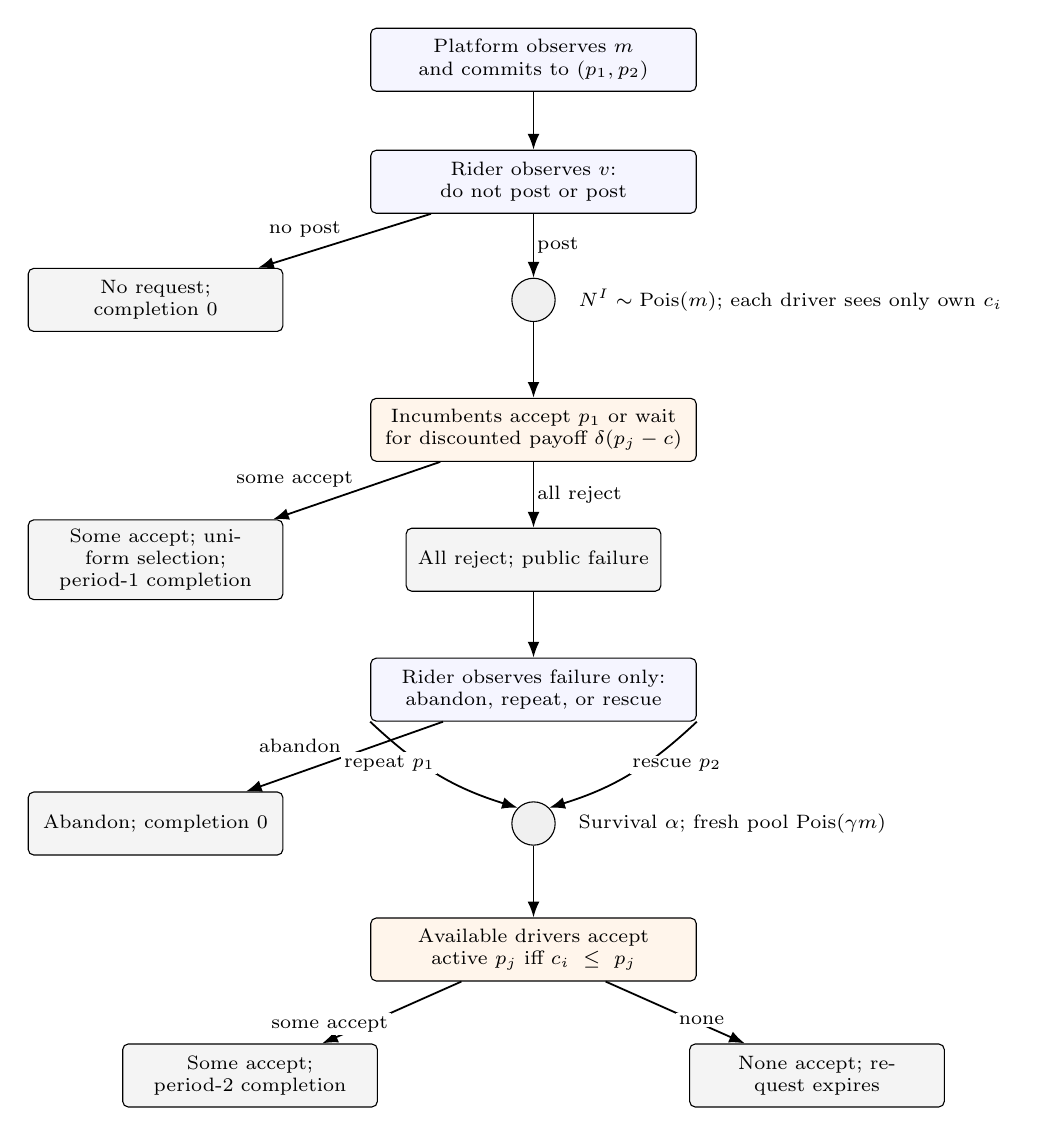
\begin{tikzpicture}[
  x=1cm,y=1cm,>={Latex[length=2mm]},
  flow/.style={->,line width=.65pt},
  box/.style={draw,rounded corners=2pt,align=center,minimum height=8mm,
    text width=39mm,font=\scriptsize,fill=blue!4},
  drv/.style={box,fill=orange!8},
  term/.style={box,fill=gray!9,text width=30mm},
  chance/.style={circle,draw,fill=gray!12,minimum size=5.5mm,inner sep=0pt},
  edge/.style={font=\scriptsize,fill=white,inner sep=1pt}]
\node[box] (platform) at (0,0) {Platform observes $m$ and commits to $(p_1,p_2)$};
\node[box] (rider0) at (0,-1.55) {Rider observes $v$: do not post or post};
\node[term] (nopost) at (-4.8,-3.05) {No request; completion $0$};
\node[chance] (pool) at (0,-3.05) {};
\node[align=left,font=\scriptsize,anchor=west] at (.45,-3.05)
 {$N^I\sim\mathrm{Pois}(m)$; each driver sees only own $c_i$};
\node[drv] (drivers1) at (0,-4.7) {Incumbents accept $p_1$ or wait for discounted payoff $\delta(p_j-c)$};
\node[term] (done1) at (-4.8,-6.35) {Some accept; uniform selection; period-1 completion};
\node[term] (fail) at (0,-6.35) {All reject; public failure};
\node[box] (rider1) at (0,-8.0) {Rider observes failure only: abandon, repeat, or rescue};
\node[term] (abandon) at (-4.8,-9.7) {Abandon; completion $0$};
\node[chance] (supply2) at (0,-9.7) {};
\node[align=left,font=\scriptsize,anchor=west] at (.45,-9.7)
 {Survival $\alpha$; fresh pool $\mathrm{Pois}(\gamma m)$};
\node[drv] (drivers2) at (0,-11.3) {Available drivers accept active $p_j$ iff $c_i\le p_j$};
\node[term] (done2) at (-3.6,-12.9) {Some accept; period-2 completion};
\node[term] (expire) at (3.6,-12.9) {None accept; request expires};
\draw[flow] (platform)--(rider0);
\draw[flow] (rider0)--node[edge,above left]{no post}(nopost);
\draw[flow] (rider0)--node[edge,right]{post}(pool);
\draw[flow] (pool)--(drivers1);
\draw[flow] (drivers1)--node[edge,above left]{some accept}(done1);
\draw[flow] (drivers1)--node[edge,right]{all reject}(fail);
\draw[flow] (fail)--(rider1);
\draw[flow] (rider1)--node[edge,above left]{abandon}(abandon);
\draw[flow] (rider1.south west) to[bend right=13]
 node[edge,above left]{repeat $p_1$}(supply2.north west);
\draw[flow] (rider1.south east) to[bend left=13]
 node[edge,above right]{rescue $p_2$}(supply2.north east);
\draw[flow] (supply2)--(drivers2);
\draw[flow] (drivers2)--node[edge,below left]{some accept}(done2);
\draw[flow] (drivers2)--node[edge,below right]{none}(expire);
\end{tikzpicture}}
{Reduced extensive form.  The realized incumbent count, rival costs,
survival, and fresh entry remain latent at the indicated decisions.
\label{fig:timing}}
{}
\end{figure}

The timing is as follows.
\begin{enumerate}[label=\textit{Stage \arabic*.},leftmargin=17mm,itemsep=2pt]
\item The platform observes the public state $m$ and commits to the entire
menu $(p_1,p_2)$.  The rescue payment cannot be revised after observing
failure.
\item The rider privately observes $v$ and chooses whether to post the
request.  A nonposted request yields zero completion.
\item Conditional on posting, the latent incumbent pool is realized.  Each
incumbent observes the menu and own cost but not the number or costs of rivals.
\item Incumbents simultaneously accept $p_1$ or wait.  If at least one accepts,
one acceptor is selected uniformly and the request completes in period 1.
\item If every incumbent rejects, universal rejection becomes public.  It
reveals the first-period screening event but not the realized pool size.
\item After observing failure, the rider chooses abandon, repeat $p_1$, or
activate $p_2$.
\item Each rejected incumbent independently survives with probability
$\alpha$.  Independently, a fresh unscreened pool with mean $\gamma m$ enters.
Counts, survival realizations, and entrant costs remain latent.
\item Available drivers accept the active terminal payment when it covers
their cost.  If at least one accepts, uniform selection produces period-2
completion; otherwise the request expires.
\end{enumerate}

\subsection{Equilibrium class, beliefs, and tie-breaking}

We use weak perfect Bayesian equilibrium (WPBE), restricted to anonymous,
symmetric, pure first-period driver cutoffs.  Under cutoff $a$, incumbents
below $a$ accept and those above $a$ wait.  The cutoff type accepts at an
interior or upper cutoff and rejects at the lower cutoff; this affects only a
null cost type.

The rider posts at a zero payoff when $v=p_1$, and does not post below it.
After failure, the following priority rule makes continuation single-valued.
If the maximal continuation payoff is zero, the rider repeats iff
$\beta v-p_1\ge0$ and otherwise abandons.  If repeat and rescue tie at a
strictly positive maximum, the rider chooses rescue.  Terminal drivers accept
at a zero surplus.  These rules matter when repeat has zero coverage: a
positive interval of rider types can then be indifferent between repeat and
abandon.

For $p_1<1$, posting implies the belief
$v\mid\{\text{post}\}\sim U[p_1,1]$.  Since supply is independent of value,
failure leaves this value posterior unchanged.  Poisson splitting determines
the rider's supply posterior after failure.  For a focal incumbent, Palm
conditioning leaves the number of rivals distributed as $\operatorname{Pois}(m)$.
At $(p_1,p_2)=(1,1)$, posting is a null event; we complete the off-path driver
subgame with cutoff one and define completion as zero.

\section{Equilibrium under an arbitrary announced menu}
\label{sec:equilibrium}

Fix a candidate cutoff $a\in[0,p_1]$ and define
\[
 \ph(x)=
 \begin{cases}(1-e^{-x})/x,&x>0,\\1,&x=0,\end{cases}
 \qquad
 \lambda_j(a)=m\{\alpha(p_j-a)+\gamma p_j\},
 \qquad C_j(a)=1-e^{-\lambda_j(a)}.
 \tag{1}
\]

\begin{lemma}[Poisson competition and failure posterior]
\label{lem:poisson}
Under cutoff $a$, first-period completion conditional on posting is
$1-e^{-ma}$.  A focal acceptor's expected assignment share is $\ph(ma)$,
while a focal waiting driver reaches failure against all rivals with
probability $e^{-ma}$.  Conditional on universal rejection, incumbents above
$a$ remain a Poisson marked population.  After survival and fresh entry,
terminal coverage at $p_j$ is $C_j(a)$, and an eligible focal driver's
terminal assignment share is $\ph(\lambda_j(a))$.
\end{lemma}

The assignment identity follows from
\[
 \E\left[\frac1{1+Z}\right]=\int_0^1\E[t^Z]dt
 =\frac{1-e^{-x}}x,\qquad Z\sim\operatorname{Pois}(x).
\]
Poisson marking gives independent counts below and above $a$.  Conditional on
no point below $a$, the above-$a$ process is unchanged.  This is not the law
of $N^I-1$ conditional on $N^I\ge1$.

After failure, rider payoffs from abandon, repeat, and rescue are
\[
 0,\qquad C_1(a)(\beta v-p_1),\qquad
 C_2(a)(\beta v-p_2).
\]
If $C_2>C_1$, define
\[
 v^M(a)=\frac{C_2(a)p_2-C_1(a)p_1}
 {\beta[C_2(a)-C_1(a)]};
\]
if $C_2=C_1$, put $v^M=+\infty$.  Conditional on posting, the repeat and
rescue masses are
\[
 \eta^R(a)=
 \frac{[\min\{v^M(a),1\}-p_1/\beta]^+}{1-p_1},
 \qquad
 \eta(a)=\frac{[1-v^M(a)]^+}{1-p_1},             \tag{2}
\]
and
\[
 \eta^R(a)+\eta(a)=
 \rho(p_1):=\frac{[1-p_1/\beta]^+}{1-p_1}.       \tag{3}
\]
The initial posting payoff is
\[
 (1-e^{-ma})(v-p_1)+e^{-ma}
 \max\{0,C_1(\beta v-p_1),C_2(\beta v-p_2)\},
\]
so the rider posts exactly when $v\ge p_1$.

A focal incumbent of cost $c$ obtains
\[
 A(c;a)=\ph(ma)(p_1-c)                           \tag{4}
\]
from accepting immediately and
\[
 W(c;a)=\delta\alpha e^{-ma}\left\{
 \eta^R(a)\ph(\lambda_1(a))[p_1-c]^+
 +\eta(a)\ph(\lambda_2(a))[p_2-c]^+
 \right\}                                       \tag{5}
\]
from waiting.  These are conditional on observing a posted request; the
posting mass must not multiply a driver's sequential payoff.

For $c\le p_1$, the margin $A-W$ is affine and strictly decreasing in $c$:
\[
 A(c;a)-W(c;a)=B(a)(p_1-c)-D(a),                 \tag{6}
\]
where
\[
\begin{aligned}
 B(a)&=\ph(ma)-\delta\alpha e^{-ma}
 \{\eta^R(a)\ph(\lambda_1)+\eta(a)\ph(\lambda_2)\},\\
 D(a)&=\delta\alpha e^{-ma}\eta(a)\ph(\lambda_2)(p_2-p_1).
\end{aligned}
\]
Indeed, $B(a)>0$ for $p_1>0$ because
\[
 B(a)\ge\ph(ma)-\delta e^{-ma}\ge0,
\]
with strictness from $a>0$ or, at $a=0$, from $\rho(p_1)<1$.  Hence a best
response is genuinely a cutoff.

Define the cutoff-type margin
\[
 f_m(a;p_1,p_2)=\ph(ma)(p_1-a)
 -\delta\alpha e^{-ma}\left\{
 \eta^R(a)\ph(\lambda_1)(p_1-a)
 +\eta(a)\ph(\lambda_2)(p_2-a)
 \right\}.                                      \tag{7}
\]

\begin{proposition}[Symmetric cutoff WPBE]
\label{prop:wpbe}
For $0<p_1<1$, the equilibrium cutoff set is
\[
\begin{aligned}
 \calE_m^{\alpha,\delta,\gamma}(p_1,p_2)
 =&\ \{0:f_m(0;p_1,p_2)\le0\}\\
 &\cup\{a\in(0,p_1):f_m(a;p_1,p_2)=0\}\\
 &\cup\{p_1:f_m(p_1;p_1,p_2)\ge0\}.
\end{aligned}                                    \tag{8}
\]
It is nonempty and compact.  At $p_1=0$, the only aggregate cutoff is zero
with the lower-boundary reject action; at $(1,1)$, set
$\calE_m^{\alpha,\delta,\gamma}(1,1)=\{1\}$.  Thus every feasible menu admits an
anonymous symmetric pure-cutoff WPBE.
\end{proposition}

At the upper boundary,
\[
 f_m(p_1;p_1,p_2)=
 -\delta\alpha e^{-mp_1}\eta(p_1)\ph(\lambda_2(p_1))(p_2-p_1)\le0,
\]
so $a=p_1$ is eligible precisely when the right side is zero.  Continuity of
$f_m$, the lower-boundary test, and the intermediate value theorem give
existence; endpoint limits remain eligible, proving compactness.

For $p_1<1$, completion on cutoff branch $a$ is
\[
 M_m^{\alpha,\gamma}(p_1,p_2;a)
 =(1-p_1)\left[1-e^{-ma}+e^{-ma}
 \{\eta^R(a)C_1(a)+\eta(a)C_2(a)\}\right].       \tag{9}
\]
We define the conservative value within the stated class by
\[
 \underline M_m^{\alpha,\delta,\gamma}(p_1,p_2)
 =\min_{a\in\calE_m^{\alpha,\delta,\gamma}(p_1,p_2)}
 M_m^{\alpha,\gamma}(p_1,p_2;a),                \tag{10}
\]
which is well-defined by Proposition~\ref{prop:wpbe}.  The announced value is
\[
 D_{\alpha,\delta,\gamma}^*(m)
 =\sup_{(p_1,p_2)\in\mathcal P^D}
 \underline M_m^{\alpha,\delta,\gamma}(p_1,p_2). \tag{11}
\]
We retain a supremum here; attainment will be proved for the main no-entry
baseline rather than assumed in the general model.

\section{Flat-payment benchmark}
\label{sec:flat}

\begin{proposition}[Flat policy]
\label{prop:flat}
For every $m>0$ and $p>0$, $(p,p)$ has the unique numeric cutoff $a=p$.
Its completion is
\[
 Q^F_\gamma(m,p)
 =(1-p)(1-e^{-mp})
 +e^{-mp}[1-p/\beta]^+(1-e^{-\gamma mp}).        \tag{12}
\]
Consequently
\[
 F_\gamma^*(m)=\max_{p\in[0,1]}Q^F_\gamma(m,p)  \tag{13}
\]
is attained.
\end{proposition}

For $a<p$, the flat cutoff margin factors as
\[
 (p-a)\left[\ph(ma)-\delta\alpha e^{-ma}\rho(p)
 \ph\bigl(m\{\alpha(p-a)+\gamma p\}\bigr)\right]>0,
\]
so no lower cutoff is sustainable.  At $a=p$, surviving rejectors have cost
above $p$ and do not accept the same payment later; only fresh drivers can
complete after failure, which gives (12).  Continuity on $[0,1]$ gives the
maximum in (13).

Let
\[
 \mathcal P_\gamma^F(m)=\arg\max_{p\in[0,1]}Q_\gamma^F(m,p)
 \quad\hbox{and}\quad
 p^0(m)=\frac{1+m-W_0(e^{1+m})}{m}.                       \tag{F1}
\]
Here $W_0$ is the principal real branch of the Lambert $W$ function, and
$p^0(m)$ is the unique maximizer of the first-window objective
$q_0(m,p)=(1-p)(1-e^{-mp})$.

\begin{lemma}[Geometry of optimized flat pricing]
\label{lem:flatgeometry}
For $m>0$, $\beta\in(0,1)$, and $\gamma>0$,
\[
 \mathcal P_\gamma^F(m)\subset(0,\beta)\cup\{p^0(m)\},
 \qquad 0<p^0(m)<\tfrac12.                               \tag{F2}
\]
The point $p^0(m)$ can be optimal only when $\beta<p^0(m)$.  Hence, if
$\beta\ge p^0(m)$---in particular, if $\beta\ge1/2$---every optimized flat
price is strictly below $\beta$.  The correspondence
$\mathcal P_\gamma^F(m)$ need not be single valued.
\end{lemma}

The lemma prevents a hidden uniqueness assumption in the mixed-entry result
below.  When $\beta<p^0(m)$, a low-price maximizer and $p^0(m)$ can tie for
some $\gamma>0$; the theorem therefore requires one active optimizer, not a
unique optimizer.

\section{Extension: Surviving Incumbents and Fresh Driver Entry}
\label{sec:localentry}

After universal rejection, two economically distinct sources of terminal
supply coexist.  A surviving incumbent appears with probability $\alpha$,
has already revealed a cost above the first-period cutoff, and discounts the
payoff from waiting by $\delta$.  A fresh entrant arrives at intensity
$\gamma m$, has not been screened by the first response, and evaluates the
terminal payment contemporaneously.  The resulting eligible intensity at
$p_j$ is
\[
 m\{\alpha(p_j-a)+\gamma p_j\},
\]
which records screening history rather than collapsing continuation supply
to the single total $(\alpha+\gamma)m$.  This composition effect is the focus
of the extension.  The central mixed-continuation case has
$0<\alpha<1$ and $\gamma>0$: some rejected incumbents disappear, some remain,
and new drivers enter before the terminal response window.  The cases
$\gamma=0$ or $\alpha\in\{0,1\}$ are nested boundaries, not substitutes for
the mixed case.

The general equilibrium characterization permits a sharp local comparison
with both sources present.  Fix $0<p<\beta$ and abbreviate
\[
 x=mp,\quad R=e^{-x},\quad E=e^{-\gamma x},\quad
 \sigma=\ph(x),\quad \ell=\ph(\gamma x),\quad
 \rho=\frac{1-p/\beta}{1-p}.                               \tag{L1}
\]
For $\alpha+\gamma>0$, define the limiting repeat--rescue switch and rescue
mass by
\[
 \bar v=\frac1\beta\left[p+
  \frac{1-E}{mE(\alpha+\gamma)}\right],\qquad
 \eta^0=\frac{1-\bar v}{1-p}.                              \tag{L2}
\]
At $\gamma=0$, the fraction in (L2) is zero.

\begin{theorem}[Fresh-entry local rescue]
\label{thm:localentry}
Suppose $m>0$, $0<p<\beta<1$, $0<\delta\le1$,
$0\le\alpha\le1$, $\gamma\ge0$,
$\alpha+\gamma>0$, and $\bar v<1$.  For all sufficiently small
$\varepsilon>0$, the menu $(p,p+\varepsilon)$ has a unique anonymous
symmetric cutoff WPBE, with
\[
 a_\varepsilon=p-\kappa\varepsilon+o(\varepsilon),\qquad
 \kappa=\frac{\delta R\alpha\ell\eta^0}
 {\sigma-\delta R\alpha\rho\ell}.                       \tag{L3}
\]
Every candidate cutoff is uniformly localized by
\[
 0\le p-a_\varepsilon
 \le\frac{\delta\alpha\rho}{1-\delta\alpha\rho}
 \varepsilon.                                                \tag{L4}
\]
The right derivative of completion is
\[
 \left.\frac{dM_m^{\alpha,\gamma}(p,p+\varepsilon;
 a_\varepsilon)}{d\varepsilon}\right|_{0+}
 =m(1-p)R\eta^0
 \frac{T_\delta}{\sigma-\delta R\alpha\rho\ell}>0,       \tag{L5}
\]
where
\[
 T_\delta=E(\alpha+\gamma)\sigma
 -\delta R\alpha\ell\{1-\rho+\rho E(1+\gamma)\}>0.       \tag{L6}
\]
\end{theorem}

The activity condition $\bar v<1$ says that a positive mass of riders uses
marginal rescue after failure.  It is automatic at $\gamma=0$ but substantive
with entry.  The knife edge $\bar v=1$ needs a second-order rider-mass
expansion and is not included.  For $\gamma>1$, activity cannot simply be
deleted from the sign claim: for example
\[
 x=1,\quad p=\tfrac12,\quad m=2,\quad \beta=\tfrac{51}{100},
 \quad\alpha=1,\quad\gamma=10,\quad\delta=\tfrac12
\]
has $\bar v>1$ and makes $T_\delta$ in (L6) negative.  Thus the
theorem's restriction is economically and mathematically real.

For $p<\beta$, define the activity index
\[
 \mathcal A_{\alpha,\gamma}(p)
 =m e^{-\gamma mp}(\alpha+\gamma)(\beta-p)
  -(1-e^{-\gamma mp}).                                   \tag{L7}
\]
Then $\mathcal A_{\alpha,\gamma}(p)>0$ is equivalent to $\bar v<1$, or
equivalently
\[
 \alpha>
 \frac{e^{\gamma mp}-1}{m(\beta-p)}-\gamma.              \tag{L8}
\]

\begin{theorem}[Optimized-flat dominance with mixed continuation supply]
\label{thm:optimizedflatentry}
Fix $m>0$, $\beta\in(0,1)$, $\delta\in(0,1]$,
$0<\alpha<1$, and $\gamma>0$.  Suppose that some
$p^*\in\mathcal P_\gamma^F(m)$ satisfies
\[
 p^*<\beta,\qquad \mathcal A_{\alpha,\gamma}(p^*)>0.      \tag{L9}
\]
For every sufficiently small $\varepsilon>0$, the menu
$(p^*,p^*+\varepsilon)$ has a unique anonymous symmetric pure-cutoff WPBE and
\[
 \underline M_m^{\alpha,\delta,\gamma}
 (p^*,p^*+\varepsilon)
 =F_\gamma^*(m)+\Lambda(p^*)\varepsilon+o(\varepsilon),
 \qquad \Lambda(p^*)>0.                                  \tag{L10}
\]
Consequently,
\[
 D_{\alpha,\delta,\gamma}^*(m)>F_\gamma^*(m).             \tag{L11}
\]
Neither uniqueness of the flat optimizer nor attainment of the general
dynamic-policy supremum is required.

If instead $p<\beta$ and $\mathcal A_{\alpha,\gamma}(p)<0$, then for every
sufficiently small $\varepsilon>0$ the same-price perturbation
$(p,p+\varepsilon)$ has the unique cutoff $a=p$, no rider activates rescue,
and its completion equals $Q_\gamma^F(m,p)$ exactly.  No first-order claim is
made at the knife edge $\mathcal A_{\alpha,\gamma}(p)=0$.
\end{theorem}

The coefficient $\Lambda(p^*)$ is the expression in (L5), evaluated at
$p=p^*$.  Condition (L9) has a direct behavioral interpretation: after flat
failure, even the highest rider type must strictly prefer access to the
marginally broader rescue pool over repeating $p^*$.  More fresh entrants do
not make this condition automatic, because entry also raises repeat coverage.

Two different quantities can reasonably be called ``the amount'' of
continuation supply.  Conditional on universal rejection at the flat cutoff
$a=p$, the expected number of second-window potential drivers is
\[
 m\tau_p,\qquad \tau_p=\alpha(1-p)+\gamma.                \tag{L12}
\]
By contrast, holding the cutoff fixed, the number made newly eligible by a
small payment increase has slope
\[
 \left.\frac1m\frac{\partial\lambda_2}{\partial p_2}
 \right|_{a=p}=\alpha+\gamma.                             \tag{L13}
\]
The next result fixes each measure in turn at the flat benchmark.  These are
local comparisons, not equal-baseline optimized-policy rankings.  Along the
equilibrium response $a_\varepsilon=p-\kappa\varepsilon+o(\varepsilon)$, raw
headcount changes at rate $m\alpha\kappa$, and terminal eligible intensity
changes at rate $m\{\alpha(1+\kappa)+\gamma\}$.  The composition response is
precisely why neither baseline normalization removes strategic waiting.

\begin{theorem}[Supply composition and strategic waiting]
\label{thm:composition}
Fix $m>0$, $0<p<\beta<1$, and $\delta\in(0,1]$, and consider
$(p,p+\varepsilon)$.

\textit{(i) Fixed continuation headcount.}  Fix $h>0$ and set
\[
 \gamma_h(\alpha)=h-(1-p)\alpha,\qquad
 A_h(\alpha)=\alpha+\gamma_h(\alpha)=h+p\alpha           \tag{L14}
\]
for $0\le\alpha\le\min\{1,h/(1-p)\}$.  This holds the conditional
headcount in (L12) fixed at $mh$.  Define
\[
 \ell_h(\alpha)=\ph(\gamma_h(\alpha)mp),\qquad
 \eta_h(\alpha)=\frac{1}{1-p}\left[
 1-\frac1\beta\left\{p+
 \frac{e^{\gamma_h(\alpha)mp}-1}{mA_h(\alpha)}\right\}
 \right].                                                 \tag{L15}
\]
On every interval on which $\eta_h(\alpha)>0$, the unique local cutoff is
\[
 a_\varepsilon(\alpha)
 =p-\kappa_h(\alpha)\varepsilon+o(\varepsilon),
 \quad
 \kappa_h(\alpha)=
 \frac{\delta e^{-mp}\alpha\ell_h(\alpha)\eta_h(\alpha)}
 {\ph(mp)-\delta e^{-mp}\alpha\rho(p)\ell_h(\alpha)},   \tag{L16}
\]
and $\kappa_h(\alpha)$ is strictly increasing in $\alpha$.

\textit{(ii) Fixed price-marginal capacity.}  Fix $s>0$ and set
\[
 \gamma_s(\alpha)=s-\alpha,\qquad
 0\le\alpha\le\min\{1,s\}.                              \tag{L17}
\]
This holds (L13) fixed at $s$.  With
\[
 \ell_s(\alpha)=\ph((s-\alpha)mp),\qquad
 \eta_s(\alpha)=\frac{1}{1-p}\left[
 1-\frac1\beta\left\{p+
 \frac{e^{(s-\alpha)mp}-1}{ms}\right\}
 \right],                                                 \tag{L18}
\]
the analogous coefficient
\[
 \kappa_s(\alpha)=
 \frac{\delta e^{-mp}\alpha\ell_s(\alpha)\eta_s(\alpha)}
 {\ph(mp)-\delta e^{-mp}\alpha\rho(p)\ell_s(\alpha)}   \tag{L19}
\]
is strictly increasing on the active set $\eta_s(\alpha)>0$.

Thus, within the active local-rescue region, replacing unscreened entrants
with screened surviving incumbents strictly increases the first-order
acceptance-erosion coefficient under either fixed-supply comparison.
\end{theorem}

The composition effect on completion is subtler than the cutoff effect.

\begin{theorem}[Closed-form endpoint boundary for local rescue value]
\label{thm:compositionvalue}
Fix $0<s\le1$, impose $\alpha+\gamma=s$, and suppose the all-entrant
composition is active:
\[
 p+\frac{e^{smp}-1}{ms}<\beta.                            \tag{L20}
\]
Let $L_s(\alpha)$ denote the right derivative in (L5) at composition
$(\alpha,s-\alpha)$.  Write
\[
 x=mp,\quad R=e^{-x},\quad E_s=e^{-sx},\quad
 \sigma=\ph(x),\quad \rho=\frac{1-p/\beta}{1-p},
\]
\[
 \eta_E=\frac{1}{1-p}\left[
 1-\frac1\beta\left\{p+\frac{e^{sx}-1}{ms}\right\}
 \right],\qquad H=\frac{E_s\eta_E}{\rho}.                \tag{L21}
\]
Then $0<H<1$ and the all-entrant and all-incumbent values are
\[
 L_s(0)=m(1-p)RsE_s\eta_E,\qquad
 L_s(s)=m(1-p)Rs\rho
 \frac{\sigma-\delta R}{\sigma-\delta Rs\rho}.           \tag{L22}
\]
Define
\[
 \delta_c(m,p,\beta,s)=
 \frac{\sigma(1-H)}{R(1-Hs\rho)}.                        \tag{L23}
\]
For $\delta\in(0,1]$,
\[
\begin{cases}
 L_s(s)>L_s(0),&\delta<\delta_c(m,p,\beta,s),\\
 L_s(s)=L_s(0),&\delta=\delta_c(m,p,\beta,s),\\
 L_s(s)<L_s(0),&\delta>\delta_c(m,p,\beta,s).
\end{cases}                                               \tag{L24}
\]
Hence the two pure compositions have generically different marginal
completion values, but their ranking depends on incumbent patience;
$L_s(\alpha)$ need not be monotone between the endpoints.
\end{theorem}

The nonmonotonicity is not a logical possibility only.  At
$(m,p,\beta,\delta,s)=(1,0.1,0.5,1,1)$, direct evaluation of the exact local
formula at three strictly mixed compositions gives approximately
\[
 L_s(0.75)=0.24267,\qquad L_s(0.92)=0.20589,\qquad
 L_s(0.99)=0.22333.                                      \tag{L25}
\]
Thus local completion value first falls and then rises with the incumbent
share even though cutoff erosion rises throughout.  This counterexample and
the activity boundary are included in the numerical falsification tests.

\section{Global menu design without fresh entry}
\label{sec:global}

We now solve the primary baseline
\[
 \gamma=0,\qquad m>0,\qquad \alpha\in(0,1],\qquad
 \beta\in(0,1),\qquad \delta\in(0,1].
\]
Let $k=\alpha m$.  Menus with $p_1\ge\beta$ or
$p_2\ge\beta$ cannot induce positive-mass rescue and are outcome-equivalent to
the flat first payment.  The nontrivial region is therefore
$0\le p_1<p_2<\beta$.

For $a\in[0,p_1]$, put
\[
 C(x)=1-e^{-kx},\qquad
 h(a)=\begin{cases}(e^{ma}-1)/a,&a>0,\\m,&a=0,\end{cases}   \tag{14}
\]
and
\[
 A_z(a)=(\beta-z)C(z-a),\quad z\in\{p_1,p_2\},
 \qquad B_1=\beta(1-p_1).                                  \tag{15}
\]
The repeat--rescue switch lies below one exactly when
$A_{p_2}(a)>A_{p_1}(a)$.
Substitution of the switch type into continuation coverage gives the exact
cancellation
\[
 K_{12}(a)
 =\frac{\max\{A_{p_1}(a),A_{p_2}(a)\}}{B_1}.               \tag{16}
\]
Multiplying the cutoff driver's payoff margin by the positive factor
$me^{ma}$ gives the sign-equivalent scalar
\[
 \mathcal D_{12}^{\delta}(a)
 =(p_1-a)h(a)-\delta K_{12}(a).                            \tag{17}
\]

The repeat branch cannot contain a cutoff below $p_1$:
\[
 (p_1-a)h(a)>\frac{A_{p_1}(a)}{B_1}
 \ge\delta\frac{A_{p_1}(a)}{B_1},\qquad 0\le a<p_1.       \tag{18}
\]
For $a>0$, this is $\ph(ma)>e^{-ma}$ combined with
$\alpha\rho(p_1)\ph(k(p_1-a))\le1$; at $a=0$, strictness follows from
$\rho(p_1)<1$.  Hence every zero of (17) under a strict active menu lies on the
rescue branch, not at the rider kink.

\begin{theorem}[Global cutoff uniqueness]
\label{thm:unique}
Fix $0\le p_1<p_2<\beta$.  If $\mathcal D_{12}^{\delta}(0)\le0$, the unique numeric
cutoff is the lower-boundary cutoff $a=0$.  If
$\mathcal D_{12}^{\delta}(0)>0$, there is a unique cutoff $a\in(0,p_1)$.  Equality at
zero never coexists with a positive root.  Together with the flat,
repeat-only, $p_1=0$, and $\alpha=0$ boundary cases, every no-entry menu has a
unique numeric symmetric cutoff under the stated cutoff-type convention.
\end{theorem}

The one-crossing argument is global.  At an active-rescue zero write
$u=p_1-a$, $z=p_2-a$, $b=\beta-p_2$, and $B=\beta(1-p_1)$.
The root equation is
\[
 uh(a)=\delta\frac bB C(z).
\]
Since $B-b=p_2-\beta p_1>0$ and $h(a)\ge m$, $u<C(z)/m$.  For
$R(a)=u h(a)/C(z)$,
\[
 \frac{R'(a)}{R(a)}
 =-\frac1u+\frac{h'(a)}{h(a)}+\frac{k}{e^{kz}-1}<0,          \tag{19}
\]
because
\[
 \frac1u-\frac{k}{e^{kz}-1}
 >m\frac{1-\alpha e^{-kz}}{1-e^{-kz}}
 \ge m>\frac{h'(a)}{h(a)}.
\]
Thus every zero crosses downward.  Since
$\mathcal D_{12}^{\delta}(p_1)<0$, two zeros would require an intervening upward
crossing.  At $p_1=0$, the numeric cutoff is zero and the cost-zero type uses
the lower-boundary reject action.

\subsection{Completion identity and comparison with the same flat payment}

At any positive cutoff, indifference gives
\[
 e^{-ma}K_{12}(a)=\frac{m\ph(ma)(p_1-a)}\delta.
\]
Using $1-e^{-ma}=ma\ph(ma)$ in (9) yields
\[
 M_m^{\alpha,\delta,0}(p_1,p_2;a)
 =(1-p_1)m\ph(ma)\left[a+\frac{p_1-a}\delta\right],
 \qquad a>0.                                                \tag{20}
\]
At a reject-all equilibrium,
\[
 M_m^{\alpha,\delta,0}(p_1,p_2;0)=
 \left(1-\frac {p_2}\beta\right)(1-e^{-kp_2})
 \ge\frac{(1-p_1)mp_1}{\delta},                           \tag{21}
\]
with equality exactly at the lower-boundary indifference condition.  Repeat
may be used by positive mass in (21); its contribution cancels algebraically.

Both $\ph(ma)$ and $a+(p_1-a)/\delta$ weakly decrease in $a>0$, and the
first decreases strictly, so (20) decreases with the cutoff.
Theorem~\ref{thm:unique} then gives a particularly strong comparison.  For
every $0<p_1<p_2<\beta$, the strict-menu cutoff is below $p_1$, and therefore
\[
 \underline M_m^{\alpha,\delta,0}(p_1,p_2)>F_m(p_1)
 =(1-p_1)(1-e^{-mp_1}).                                    \tag{22}
\]
This is a global same-$p_1$ result, not merely a derivative along one selected
branch.

For completeness, a one-sided local expansion at $(p_1,p_1)$ is
\[
 a_\varepsilon=p_1-\kappa\varepsilon+o(\varepsilon),
 \qquad
 \kappa=
 \frac{\delta e^{-mp_1}\alpha\rho(p_1)}
 {\ph(mp_1)-\delta e^{-mp_1}\alpha\rho(p_1)},            \tag{23}
\]
and
\[
 \left.\frac{dM(p_1,p_1+\varepsilon)}{d\varepsilon}\right|_{0+}
 =\frac{m(1-p_1)e^{-mp_1}\alpha\rho(p_1)
 [\ph(mp_1)-\delta e^{-mp_1}]}
 {\ph(mp_1)-\delta e^{-mp_1}\alpha\rho(p_1)}>0.          \tag{24}
\]
The wedge decomposes as
$\ph(mp_1)-\delta e^{-mp_1}=[\ph(mp_1)-e^{-mp_1}]
+(1-\delta)e^{-mp_1}$:
assignment competition is the first term and incumbent impatience the second.

\subsection{The fixed-first-payment problem}

Following the design sequence, fix $p_1$ before optimizing $p_2$.  For a target
cutoff $a<\beta$, maximize
\[
 A(a,p_2)=(\beta-p_2)[1-e^{-k(p_2-a)}],
 \qquad p_2\in[a,\beta].                                   \tag{25}
\]
It is strictly concave.  Its unique maximizer $Q(a)$ satisfies
\[
 e^{k(Q(a)-a)}-1=k(\beta-Q(a)),                              \tag{26}
\]
or
\[
 Q(a)=\beta-
 \frac{W_0(e^{1+k(\beta-a)})-1}{k}.                         \tag{27}
\]
Moreover
\[
 a<Q(a)<\frac{a+\beta}{2}.
\]
Let
\[
 S(a)=A(a,Q(a)),\qquad
 S(a)=\frac{k[\beta-Q(a)]^2}{1+k[\beta-Q(a)]}.              \tag{28}
\]
Define $Q_0=Q(0)$, $S_0=S(0)$, and
\[
 p_z=\frac{1-\sqrt{1-4\delta S_0/(\beta m)}}2.             \tag{29}
\]
The strict flat inequality at $p_1=Q_0,a=0$ gives
$0<p_z<Q_0<1/2$.

\begin{theorem}[Optimal rescue conditional on the first payment]
\label{thm:fixedp}
Let
\[
 H_m(p_1)=\max_{p_2\in[p_1,1]}
 \underline M_m^{\alpha,\delta,0}(p_1,p_2).
\]
Then:
\begin{enumerate}[label=(\roman*)]
 \item If $0\le p_1\le p_z$, the unique optimal rescue is $p_2=Q_0$, the
 cutoff is the lower-boundary reject-all cutoff $a=0$, and
 \[
 H_m(p_1)=S_0/\beta.
 \]
 \item If $p_z<p_1<\beta$, there is a unique $a^*(p_1)\in(0,p_1)$ satisfying
 \[
 (p_1-a)h(a)=\frac{\delta S(a)}{\beta(1-p_1)}.             \tag{30}
 \]
 The unique optimal rescue is $p_2=Q(a^*(p_1))$, and
 \[
 H_m(p_1)=(1-p_1)m\ph(ma^*(p_1))
 \left[a^*(p_1)+\frac{p_1-a^*(p_1)}\delta\right].
 \]
 \item If $\beta\le p_1\le1$, every $p_2\in[p_1,1]$ is outcome-equivalent and
 \[
 H_m(p_1)=(1-p_1)(1-e^{-mp_1}).
 \]
\end{enumerate}
Thus the conditional supremum is a maximum in every regime.
\end{theorem}

To see implementability, a positive target cutoff solves
\[
 A(a,p_2)=\frac{\beta(1-p_1)(p_1-a)h(a)}\delta.           \tag{31}
\]
The right side strictly exceeds $A(a,p_1)$ by (18), so (31) cannot generate a
repeat-only or kink pseudo-solution.  If the envelope is below, equal to, or
above the right side, there are respectively zero, one tangent, or two strict
implementing prices.  Theorem~\ref{thm:unique} makes each implemented cutoff
the unique equilibrium.  Completion falls with the cutoff, so the smallest
implementable cutoff, attained at tangency, solves the fixed-$p_1$ problem.

\subsection{One-dimensional global design and attainment}

Define
\[
 R_\delta(a)=\frac{\delta S(a)}{\beta h(a)}.
\]
The tangent equation is
\[
 (1-p_1)(p_1-a)=R_\delta(a).                               \tag{32}
\]
Because $Q(a)<(1+a)/2$ and the left side is increasing in $p_1$ below that
vertex, the unique feasible root is the lower quadratic branch
\[
 P_\delta(a)=
 \frac{1+a-\sqrt{(1-a)^2-4R_\delta(a)}}2.                  \tag{33}
\]
The upper branch is not a fixed-$p_1$ rescue optimum.  The map $P_\delta$ is
continuous and strictly increasing from $[0,\beta]$ onto $[p_z,\beta]$.
Endpoint injectivity follows from the same envelope one-crossing argument:
$P_\delta(a)=P_\delta(0)=p_z$ for $a>0$ would give the fixed-$p_1=p_z$
envelope two zeros.

Extend $P_\delta(\beta)=Q(\beta)=\beta$ and set
\[
 J_\delta(a)=
 \begin{cases}
 (1-P_\delta(a))m\ph(ma)
 \left[a+\dfrac{P_\delta(a)-a}\delta\right],&a>0,\\[6pt]
 mp_z(1-p_z)/\delta=S_0/\beta,&a=0.
 \end{cases}                                                \tag{34}
\]
Then $J_\delta(\beta)=(1-\beta)(1-e^{-m\beta})$, and the complete outer
problem is
\[
 D_{\alpha,\delta,0}^*(m)=
 \max\left\{
 \max_{a\in[0,\beta]}J_\delta(a),
 \max_{p\in[\beta,1]}(1-p)(1-e^{-mp})
 \right\}.                                                  \tag{35}
\]

\begin{theorem}[Policy attainment and optimized-flat dominance]
\label{thm:global}
For every no-entry parameter tuple with $m>0$ and $\alpha>0$, the announced
policy value in (11) is attained.  If $\beta\ge1/2$, every optimal menu is a
strict menu
\[
 (p_1^*,p_2^*)=(P_\delta(a^*),Q(a^*)),
 \qquad a^*\in\argmax_{a\in[0,\beta]}J_\delta(a)
 \subset(0,\beta),                                          \tag{36}
\]
and
\[
 D_{\alpha,\delta,0}^*(m)>F_0^*(m).                         \tag{37}
\]
No uniqueness of $a^*$ is asserted.
\end{theorem}

Equation (35) is a maximum of continuous functions on compact intervals, so
it proves attainment directly.  In the no-entry flat problem,
\[
 F_m(p)=(1-p)(1-e^{-mp})
\]
is strictly concave and its unique optimizer is
\[
 p_F(m)=\frac{1+m-W_0(e^{1+m})}{m}<\frac12.                 \tag{38}
\]
For $\beta\ge1/2$, $p_F<\beta$, and (22) applied at $p_F$ proves (37),
including the equality case $\beta=1/2$.  The boundary portions of (35) do
not beat $F_0^*$, whereas (37) does, so every global optimizer is interior and
strict.

The driver discount also yields a clean comparative static.  Write
$R_1(a)=S(a)/[\beta h(a)]$, so that
$(1-P_\delta)(P_\delta-a)=\delta R_1(a)$.  For
$a\in(0,\beta)$,
\[
 \frac{\partial P_\delta(a)}{\partial\delta}
 =\frac{R_1(a)}{1+a-2P_\delta(a)}>0,
 \qquad
 \frac{\partial J_\delta(a)}{\partial\delta}
 =-(1-e^{-ma})
 \frac{\partial P_\delta(a)}{\partial\delta}<0.            \tag{38a}
\]
Thus $D_{\alpha,\delta,0}^*(m)$ is weakly decreasing in $\delta$: more
patient incumbents require a higher first payment to implement the same
cutoff and continuation coverage.  This is a completion comparative static,
not a welfare ranking.

\subsection{The full patience region}

Fix $(m,\alpha,\delta)$ and make patience explicit in $D(m;\beta)$.  For a fixed
strict menu $p_1<p_2$, its value equals $F_m(p_1)$ for $\beta\le p_2$ and is
strictly increasing for $\beta>p_2$.  Indeed, increasing $\beta$ raises the active-rescue
coefficient in (17), shifts the unique cutoff strictly left (or to zero), and
then raises completion by (20)--(21).

The scalar representation is jointly continuous in patience.  To use a fixed
choice set, write $a=\beta x$.  The solution of
\[
 e^{ky}-1=k\{\beta(1-x)-y\}
\]
is continuous in $(\beta,x)$.  At $x=0$, $h(0)=m$ and
$P_{\beta,\delta}(0)=p_z(\beta)$ has a strictly positive discriminant; at
$x=1$, $P_{\beta,\delta}(\beta)=Q_\beta(\beta)=\beta$ and
$J_{\beta,\delta}(\beta)=(1-\beta)(1-e^{-m\beta})$.  These removable extensions and
the elementary maximum theorem make $D(m;\beta)$ continuous.

Define
\[
 \beta_c(m,\alpha,\delta)=
 \inf\{\beta\in(0,1):D_{\alpha,\delta,0}^*(m;\beta)>F_0^*(m)\}. \tag{39}
\]

\begin{theorem}[Patience threshold]
\label{thm:patience}
For $m>0$, $0<\alpha\le1$, and $0<\delta\le1$, the strict-gain region is the single upper
interval
\[
 D_{\alpha,\delta,0}^*(m;\beta)>F_0^*(m)
 \quad\Longleftrightarrow\quad
 \beta>\beta_c(m,\alpha,\delta).                           \tag{40}
\]
Moreover
\[
 0< -\frac1m\log(1-F_0^*(m))
 \le\beta_c(m,\alpha,\delta)\le p_F(m)<\frac12.           \tag{41}
\]
For fixed $(m,\alpha,\delta)$, $D(m;\beta)=F_0^*(m)$ through the threshold and is
strictly increasing above it.  The exact scalar test is
\[
 \beta>\beta_c(m,\alpha,\delta)
 \quad\Longleftrightarrow\quad
 \max_{a\in[0,\beta]}J_{\beta,\delta}(a)>F_0^*(m).        \tag{42}
\]
When $\alpha=0$, the gain region is empty.
\end{theorem}

Pointwise monotonicity in (38a) also nests the thresholds:
\[
 0<\delta_1<\delta_2\le1
 \quad\Longrightarrow\quad
 \beta_c(m,\alpha,\delta_1)
 \le\beta_c(m,\alpha,\delta_2).                            \tag{42a}
\]
Strict inequality is not asserted globally.

The lower bound follows because an active menu has $p_2<\beta$ and completion
requires an initial incumbent with cost at most $p_2$, giving
$M<1-e^{-m\beta}$.  The upper bound follows from a strict menu at $p_F$ when
$\beta>p_F$.  If gain holds at one patience level, attainment supplies an
optimal strict menu; reusing it at any larger $\beta$ and applying the fixed
menu monotonicity gives strict gain and strict value increase.  Continuity
makes the gain interval open.

\section{Market thickness: topology and endpoint rates}
\label{sec:thickness}

Fix $0<\alpha\le1$, $0<\beta<1$, $0<\delta\le1$, and $\gamma=0$.  Holding
these primitives and the same thickness $m$ fixed, define
\[
 M_R^*(m):=D_{\alpha,\delta,0}^*(m),\qquad
 M_F^*(m):=F_0^*(m),\qquad
 V(m):=M_R^*(m)-M_F^*(m).                                 \tag{43}
\]
Thus $V(m)$ is the completion-rate gain from allowing an optimally designed
rescue menu instead of an optimally chosen flat payment at the same market
thickness.  It is not the marginal value of adding drivers; $100V(m)$ is the
gain in percentage points.
The outer representation (35), rather than a local-menu derivative, is the
appropriate object because the optimal menu moves with thickness.

For the thin limit, define on $a\in[0,\beta]$
\[
 P_0^\delta(a)=
 \frac{1+a-\sqrt{(1-a)^2-
 \delta\alpha(\beta-a)^2/\beta}}2,
 \qquad
 H_0^\delta(a)=a[1-P_0^\delta(a)]
 +\frac{\alpha(\beta-a)^2}{4\beta},                       \tag{44}
\]
and $G_{\alpha,\beta,\delta}=\max_{a\in[0,\beta]}H_0^\delta(a)$.

\begin{theorem}[Thickness topology and exact endpoint regimes]
\label{thm:thickness}
For fixed $(\alpha,\beta,\delta)\in(0,1]\times(0,1)\times(0,1]$:
\begin{enumerate}[label=(\roman*)]
 \item $M_R^*(m)$, $M_F^*(m)$, and $V(m)$ are continuous on
 $(0,\infty)$.  The scalar
 cutoff and flat-price argmax correspondences are nonempty, compact valued,
 and upper hemicontinuous.

 \item If $\beta>1/2$ and $\delta<1$, then
 \[
  V(m)
  \sim\left(G_{\alpha,\beta,\delta}-\frac14\right)m,
  \qquad G_{\alpha,\beta,\delta}>\frac14.                 \tag{45}
 \]
 At the no-discount boundary $\delta=1$, let $a_0\in(0,1/2)$ be the
 unique solution of
 \[
  \alpha(\beta-a_0)^2=\beta(1-2a_0).
 \]
 Then
 \[
  V(m)\sim\frac{1-2a_0}{16}m^2.                           \tag{46}
 \]

 \item If $\beta=1/2$ and $\delta<1$, then
 \[
  V(m)
  \sim
  \frac{\alpha(1-\delta)}
  {512\{1-\alpha(1-\delta)/2\}}m^3.                       \tag{47}
 \]
 At $\delta=1$, the leading cancellation persists one order longer:
 \[
  V(m)\sim\frac{\alpha}{2048}m^4.                         \tag{48}
 \]

 \item If $\beta<1/2$, there exists
 $m_0(\alpha,\beta,\delta)>0$ such that
 \[
  M_R^*(m)=M_F^*(m),\qquad
  V(m)=0,
  \qquad 0<m<m_0(\alpha,\beta,\delta).                   \tag{49}
 \]

 \item As $m\to\infty$,
 \[
  1-M_R^*(m)\sim\frac{\log\log m}{m},
  \quad 1-M_F^*(m)\sim\frac{\log m}{m},
  \quad V(m)\sim\frac{\log m}{m}.                        \tag{50}
 \]
 For each fixed positive $(\alpha,\beta)$, the estimates establishing (50)
 are uniform over the full policy/cutoff domain and uniformly over
 $\delta\in(0,1]$.  They are not uniform over primitive sequences with
 $\alpha\downarrow0$ or $\beta\downarrow0$.
\end{enumerate}
\end{theorem}

Equations (45)--(48) show a singular boundary: the limits $m\downarrow0$ and
$\delta\uparrow1$ do not commute at the first nonzero order.  Even slight
incumbent impatience creates a first-order screening gain when $\beta>1/2$
and a cubic gain at $\beta=1/2$; exact patience removes those terms.

Here is the proof architecture.  Let $k=\alpha m$ and let $z_m(a)$ solve
\[
 z_m(a)+\log[1+z_m(a)]=k(\beta-a),
 \qquad y_m(a)=z_m(a)/k.
\]
Then
\[
 Q_m(a)=\beta-y_m(a),\quad
 T_m(a)=\frac{k y_m(a)^2}{\beta[1+k y_m(a)]},\quad
 B_m^\delta(a)=\delta\frac{a}{e^{ma}-1}T_m(a),             \tag{51}
\]
with $a/(e^{ma}-1)=1/m$ at zero, and
\[
 P_m^\delta(a)=
 \frac{1+a-\sqrt{(1-a)^2-4B_m^\delta(a)}}2.               \tag{52}
\]
The scalar objective admits the useful exact form
\[
 J_m^\delta(a)
 =[1-P_m^\delta(a)](1-e^{-ma})+T_m(a)e^{-ma}.              \tag{53}
\]
The strict envelope bound keeps the discriminant positive.  Joint
continuity and Berge's maximum theorem prove part (i).

Uniformly on $[0,\beta]$, $P_m^\delta\to P_0^\delta$ and
$J_m^\delta/m\to H_0^\delta$.  If $\beta>1/2$ and $\delta<1$, the unique
$a\in(0,1/2)$ satisfying $P_0^\delta(a)=1/2$ gives
\[
 H_0^\delta(a)=\frac12\left[a+\frac{1/2-a}{\delta}\right]
 >\frac14,
\]
which proves the strict coefficient in (45); uniform convergence gives its
exact value as the maximum in (44).  For $\delta=1$, the first-order term
ties the flat benchmark, and the uniform second-order argmax expansion gives
(46).

At $\beta=1/2$, every thin optimizer localizes as $a=1/2-cm$.  Put
$A_\delta=1-\alpha(1-\delta)/2$.  Uniformly for bounded $c$,
\[
 J_m^\delta(1/2-cm)
 =\frac m4-\frac{m^2}{16}
 +m^3\left\{\frac1{96}+\frac c8-A_\delta c^2\right\}
 +O(m^4).                                                   \tag{54}
\]
The maximizing rescaled cutoff is $c^*=1/(16A_\delta)$, while the flat
$m^3$ coefficient is $11/768$.  Their difference is exactly the coefficient
in (47).  When $\delta=1$ it vanishes; the fourth-order expansion yields
(48).  In particular, uniformly for bounded $c$,
\[
 \begin{aligned}
 J_m^1(1/2-cm)
 &=\frac m4-\frac{m^2}{16}+m^3 f_2(c)+m^4 f_3(c)+o(m^4),\\
 f_2(c)&=\frac{11}{768}-\left(c-\frac1{16}\right)^2,\\
 f_3(c)&=-\frac1{768}-\frac c{24}+\frac{c^2}{4}+2\alpha c^3,
 \end{aligned}                                             \tag{54a}
\]
whereas
\[
 F_0^*(m)=\frac m4-\frac{m^2}{16}
 +\frac{11}{768}m^3-\frac3{1024}m^4+o(m^4).              \tag{54b}
\]
The strict quadratic loss in $f_2$ and local Lipschitz control of $f_3$
evaluate the perturbed maximum at $c=1/16$ to fourth order, and
$f_3(1/16)=-3/1024+\alpha/2048$.  Subtracting (54b) proves (48).
If $\beta<1/2$, the bound
\[
 H_0^\delta(a)
 \le a(1-a)+\frac{(\beta-a)^2}{4\beta}
 \le\beta(1-\beta)<\frac14
\]
is uniform on $[0,\beta]$.  Since the flat optimizer converges to $1/2$,
the flat policy wins exactly on a nonempty initial interval, proving (49).

For the thick limit put $x=ma$, $p_1=P_m^\delta(a)$, and $T=T_m(a)$.  Equation
(53) gives the same exact nonnegative loss decomposition for every fixed
$\delta>0$:
\[
 1-J_m^\delta(a)=p_1(1-e^{-x})+(1-T)e^{-x}.                \tag{55}
\]
The feasible choice $x=\log\log m$ and the policy-uniform lower bound obtained
by splitting at $Q_m(a)=\beta/2$ give the first rate in (50).  The exact flat
first-order condition gives the second, and subtraction gives the third.

\begin{corollary}[A best finite thickness, without a shape theorem]
\label{cor:bestm}
For every fixed positive $(\alpha,\beta,\delta)$ in the maintained ranges,
there exists $m^*\in(0,\infty)$ such that
\[
 V(m^*)=\max_{m>0}V(m)>0.                                 \tag{56}
\]
Strict single-peakedness is false when $\beta<1/2$ because of (49).  For
$\beta\ge1/2$, strict single-peakedness remains open for every fixed
$\delta\in(0,1]$.
\end{corollary}

Continuity, endpoint vanishing, and eventual positivity in (50) localize a
global maximizer to a compact subinterval.  No uniqueness of $m^*$ is claimed.

\subsection{Theoretical numerical illustration}

Figure~\ref{fig:theoryprofiles} and Table~\ref{tab:selectedm} illustrate the
uniform model at $\alpha=1$ and $\beta=\delta=0.8$.  These values are chosen
to display the mechanism and are not empirical estimates.  Each thickness
point re-solves the equilibrium cutoff and then optimizes $p_2$ conditional on
$p_1$ before optimizing $p_1$.

\begin{figure}
\FIGURE
{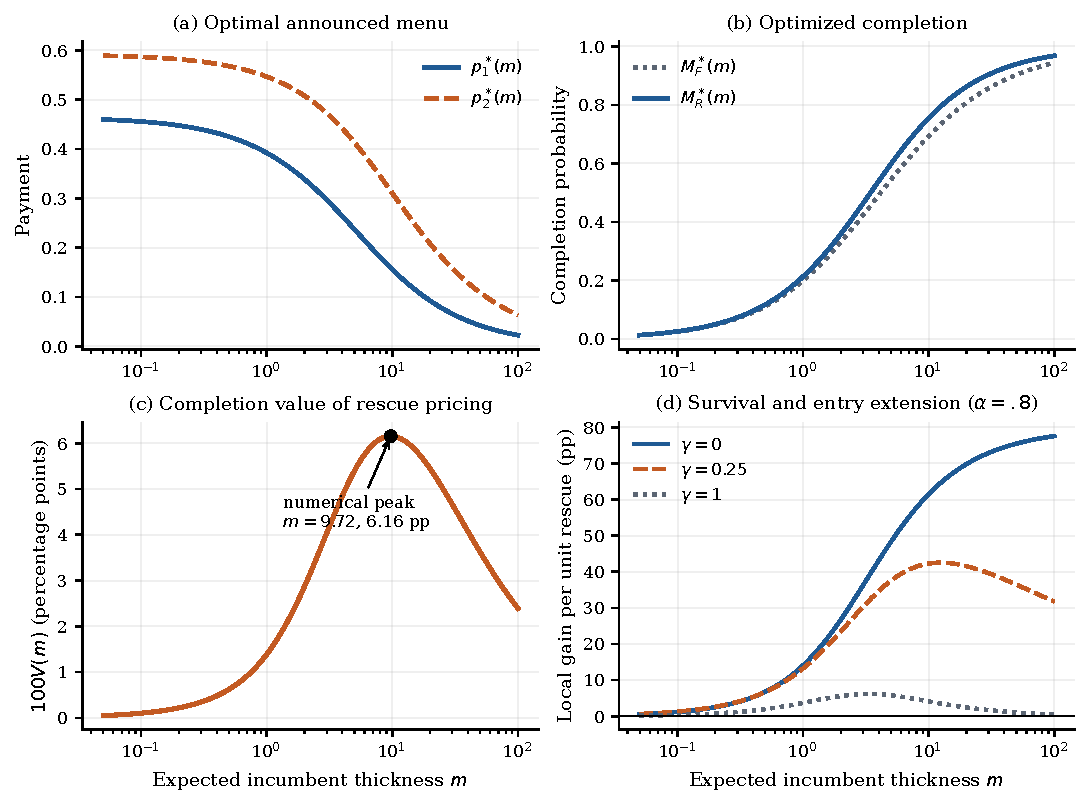
\includegraphics[width=\textwidth]{figures/theory_profiles.pdf}}
{Theoretical rescue profiles and the survival--entry extension.
Panels (a)--(c) use $\alpha=1$, $\beta=\delta=0.8$, and $\gamma=0$.
The marked point in panel (c) is a numerical maximizer, not a uniqueness
theorem.  Panel (d) fixes $\alpha=0.8$, evaluates a marginal announced rescue
at the no-entry flat benchmark, and varies fresh-entry intensity $\gamma$.
The dashed and dotted profiles have $0<\alpha<1$ and $\gamma>0$, so the
terminal pool contains both screened surviving incumbents and unscreened new
drivers; the solid $\gamma=0$ profile is the nested no-entry boundary.  Zero
local gain can reflect an inactive rescue mass.  All calculations are
model-generated and nonempirical.\label{fig:theoryprofiles}}
{}
\end{figure}

\begin{table}
\TABLE
{Selected-thickness theoretical solutions.\label{tab:selectedm}}
{\centering\begin{tabular}{rrrrrrr}
\toprule
$m$ & $p_1^*$ & $p_2^*$ & $a^*$ & $M_R^*$ & $M_F^*$ & $100V(m)$ \\
\midrule
1 & 0.3919 & 0.5464 & 0.3203 & 0.2132 & 0.1993 & 1.3883 \\
5 & 0.2369 & 0.4131 & 0.1978 & 0.5978 & 0.5438 & 5.4003 \\
10 & 0.1559 & 0.3103 & 0.1329 & 0.7552 & 0.6936 & 6.1552 \\
20 & 0.0925 & 0.2081 & 0.0804 & 0.8624 & 0.8080 & 5.4437 \\
\bottomrule
\end{tabular}
}
{Parameters are $\alpha=1$, $\beta=\delta=0.8$, and $\gamma=0$.
$a^*$ is the equilibrium first-period cutoff and $100V(m)$ is the completion
gain in percentage points.  The table is a theoretical numerical
illustration, not an empirical calibration.}
\end{table}

\section{A public-supply benchmark}
\label{sec:publicN}

The Poisson model makes realized local supply latent.  To separate that
information friction from assignment competition, fix instead a deterministic
incumbent count $n\ge1$ observed by every agent.  We evaluate one announced
menu conditional on that fixed $n$; the exercise removes rival-count
uncertainty without introducing state-contingent pricing.  Keep the timing,
uniform private costs, survival, and no-entry assumption.
For a conjectured cutoff $a$, a focal acceptor faces
$X\sim\operatorname{Bin}(n-1,a)$ accepting rivals, so her assignment share is
\[
 s_n(a):=\E\!\left[\frac1{1+X}\right]
 =\frac{1-(1-a)^n}{na},
 \qquad s_n(0)=1.                                           \tag{57}
\]
Universal rejection occurs against all of her rivals with probability
$(1-a)^{n-1}$.  Conditional on that event, each rival has cost uniform on
$(a,1)$.  If terminal payment $p_j$ is selected, a rival is both surviving
and eligible with probability
\[
 \theta_j(a)=\frac{\alpha(p_j-a)}{1-a};
\]
hence a terminal acceptor's assignment share is $s_n(\theta_j)$ and terminal
coverage is
\[
 C_{j,n}(a)=1-[1-\theta_j(a)]^n
           =n\theta_j(a)s_n(\theta_j(a)).                   \tag{58}
\]

Let $\eta_j(a)$ be the posting-conditional mass of riders who select terminal
payment $p_j$ after failure.  At a positive interior cutoff, indifference of
the cutoff driver is
\[
 s_n(a)(p_1-a)
 =\delta(1-a)^{n-1}\alpha
   \sum_j\eta_j(a)s_n(\theta_j(a))(p_j-a).                  \tag{59}
\]
Substitution of (58)--(59) into unconditional completion gives the exact
finite-population counterpart of (20):
\[
 M_n(p_1,p_2;a)
 =(1-p_1)n s_n(a)\left[a+\frac{p_1-a}\delta\right].       \tag{60}
\]

\begin{proposition}[Public $n$ and local announced rescue]
\label{prop:publicN}
Fix $n\ge1$, $0<\alpha\le1$, $0<\delta\le1$, and
$p\in(0,\beta)$.  For every sufficiently
small $\varepsilon>0$, the menu $(p,p+\varepsilon)$ has a unique symmetric
cutoff, and it satisfies
\[
 a_\varepsilon=p-\kappa_n\varepsilon+o(\varepsilon),
 \qquad
 \kappa_n=
 \frac{\delta(1-p)^{n-1}\alpha\rho(p)}
 {s_n(p)-\delta(1-p)^{n-1}\alpha\rho(p)}>0.                \tag{61}
\]
Its right derivative of unconditional completion is
\[
 \left.\frac{dM_n}{d\varepsilon}\right|_{0+}
 =(1-p)n\kappa_n
 \left\{\frac{1-\delta}{\delta}s_n(p)-p\,s_n'(p)\right\}. \tag{62}
\]
This derivative is strictly positive for every $n\ge1$ when $\delta<1$.
At $\delta=1$, it is strictly positive for $n\ge2$ and exactly zero for
$n=1$.
\end{proposition}

The denominator in (61) is positive because
$s_n(p)\ge(1-p)^{n-1}$ and $\delta\alpha\rho(p)<1$.  Moreover
\[
 s_n(a)=\frac1n\sum_{r=0}^{n-1}(1-a)^r,
\]
which is strictly decreasing for $n\ge2$ and constant for $n=1$.
Proposition~\ref{prop:publicN} rules out the claim that an unobserved realized
count is necessary for the rescue gain.  The first term in (62) is pure
intertemporal compensation and survives at $n=1$; the second is assignment
competition and is positive exactly when $n\ge2$.  Latent supply changes
posterior inference and the global policy problem, but neither local wedge.
If $\alpha=0$, then $\kappa_n=0$ and the derivative in (62) is zero for
every $n$.

\section{Planned Empirical Calibration and Counterfactual Design}
\label{sec:calibration}

\paragraph{Current status.}
This section is a pre-specified empirical placeholder.  The repository does
not contain request-level observations or a protocol verifying that $p_2$ was
announced before first-period decisions.  No estimate, standard error, model
fit, or empirical counterfactual is claimed in the present version.  The
theoretical numerical illustration in Section~\ref{sec:thickness} is not an
empirical calibration.

\subsection{Parameter status and identifying variation}

Before estimation, every model object will receive exactly one status:
measured, estimated, calibrated, or fixed for sensitivity.  Table
\ref{tab:parameter-ledger} records the identifying variation required for the
main primitives.

\begin{table}
\TABLE
{Pre-specified parameter and identification ledger (design only; no estimates).\label{tab:parameter-ledger}}
{\begin{tabularx}{\textwidth}{L{16mm}L{28mm}XL{24mm}}
\toprule
Object & Planned status & Required variation or moment & Current entry\\
\midrule
$m$ & measured or estimated state & Initial eligible exposure and pre-decision supply signal & \DataRequired\\
$\alpha$ & measured or estimated & Fraction of rejected incumbents still eligible in period 2 & \DataRequired\\
$\gamma$ & measured or estimated & New period-2 eligible drivers relative to initial expected supply & \DataRequired\\
$F$ & calibrated & Acceptance by exogenous payment among exposed drivers & \DataRequired\\
$G,\beta$ & estimated or bounded & Posting and continuation across price, delay, and predicted coverage & \DataRequired\\
$\delta$ & estimated or bounded & First-period acceptance response to announced $p_2$ holding $p_1$ fixed & \DataRequired\\
\bottomrule
\end{tabularx}}
{A static price experiment can discipline contemporaneous acceptance but does
not identify $\delta$ or the announcement channel without ex ante variation in
$p_2$.  Persistent driver identifiers are required to separate $\alpha$ from
$\gamma$.}
\end{table}

The initial implementation maintains the model restriction that incumbent
and entrant costs share the same primitive distribution $F$.  A later
robustness extension may allow $F_I\ne F_E$, but doing so requires
rederiving and recomputing the equilibrium rather than relabeling the current
moments.  Even under a common primitive distribution, incumbents are selected
into the continuation pool by first-period rejection whereas entrants are
unscreened.

\subsection{Calibration criterion and equilibrium computation}

Let $\theta$ collect the empirical parameters and let $\widehat g$ contain
request-level moments.  The planned minimum-distance estimator is
\[
 \widehat\theta\in\arg\min_{\theta\in\Theta}
 [\widehat g-g(\theta)]^{\mathsf T}W
 [\widehat g-g(\theta)].                                  \tag{63}
\]
Target moments include posting, first-period acceptance, universal rejection,
abandonment, repetition, rescue activation, incumbent survival, fresh entry,
terminal acceptance, and unconditional completion.  Each evaluation of
$g(\theta)$ must resolve the cutoff-WPBE for every relevant menu and market
state.  All roots and boundary equilibria are enumerated, and the maintained
selection rule is applied before moments are aggregated.  The platform policy
is optimized only after this equilibrium step.

The estimation report will list parameter bounds, normalizations, starting
points, global and local search methods, numerical tolerances, convergence
criteria, cutoff residuals, and the weighting matrix.  Parameters not point
identified by the available variation will be reported as profiles, bounds,
or sensitivity regions rather than arbitrary point estimates.

\subsection{Fit and validation}

Targeted moments and validation moments will be separated before estimation.
When the data permit, a market, date, geography, or randomized arm will be
held out.  The principal benchmark models are flat pricing, myopic acceptance,
no anticipation of $p_2$, a model that pools incumbents and entrants, and
alternative $F_I,F_E,G$ specifications.

\begin{table}
\TABLE
{Model fit and validation placeholders (no estimates).\label{tab:fit}}
{\begin{tabularx}{\textwidth}{XL{28mm}L{28mm}L{28mm}}
\toprule
Moment & Data & Model & Use\\
\midrule
First-period acceptance & \DataRequired & \DataRequired & Target/holdout\\
Universal rejection & \DataRequired & \DataRequired & Target/holdout\\
Abandon/repeat/rescue shares & \DataRequired & \DataRequired & Target/holdout\\
Incumbent survival and fresh entry & \DataRequired & \DataRequired & Target/holdout\\
Terminal acceptance & \DataRequired & \DataRequired & Target/holdout\\
Unconditional completion & \DataRequired & \DataRequired & Target/holdout\\
\bottomrule
\end{tabularx}}
{The final table will report sample sizes, empirical uncertainty, absolute
error, and whether each moment was targeted or reserved for validation.}
\end{table}

\subsection{Policy counterfactuals}

If the data gates are satisfied, a future empirical implementation will
compare the observed policy, optimized flat pricing, optimized announced
rescue, and a no-anticipation benchmark.  The
main outcomes are $p_1^*(m)$, $p_2^*(m)$, $M_F^*(m)$, $M_R^*(m)$, $V(m)$,
first-period completion, rescue use, and delay.  The extension varies
$\alpha$, $\gamma$, $\beta$, and $\delta$ separately so that the effects of
screened surviving incumbents and unscreened entrants are not summarized by a
single continuation-supply number.

\begin{table}
\TABLE
{Counterfactual-policy placeholders (no estimates).\label{tab:counterfactual}}
{\begin{tabularx}{\textwidth}{XL{22mm}L{22mm}L{23mm}L{23mm}}
\toprule
Policy & $p_1$ & $p_2$ & Completion & Rescue use\\
\midrule
Observed/current & \DataRequired & \DataRequired & \DataRequired & \DataRequired\\
Optimized flat & \DataRequired & same as $p_1$ & \DataRequired & 0\\
Optimized announced rescue & \DataRequired & \DataRequired & \DataRequired & \DataRequired\\
No-anticipation benchmark & \DataRequired & \DataRequired & \DataRequired & \DataRequired\\
\bottomrule
\end{tabularx}}
{Completion changes will be reported in percentage points and relative to the
appropriate baseline.  Global optimization with $\gamma>0$ is numerical
evidence, not an extension of the no-entry global theorem.}
\end{table}

Sampling and parameter uncertainty will be propagated through the entire
equilibrium and policy-optimization procedure.  The resampling unit will match
the assignment and dependence structure, and parameters will be re-estimated
inside every bootstrap draw.  Confidence bands for $p_1^*(m)$, $p_2^*(m)$,
and $V(m)$ will distinguish the support of observed thickness from model
extrapolation.

\section{Managerial interpretation and institutional scope}
\label{sec:discussion}

The fixed-$p_1$ solution gives a concrete menu-design rule rather than a
generic instruction to raise payment after failure.  A sufficiently low
first payment places the request in a reject-all regime and uses the unique
rescue-envelope maximizer.  At an intermediate $p_1$, the platform chooses a
tangent rescue payment that implements the smallest feasible cutoff.  Once
$p_1$ reaches rider patience $\beta$, a separate rescue payment no longer
changes positive-mass continuation behavior.

Three state variables matter operationally.  Rider patience determines
whether delayed completion remains valuable enough to finance rescue.  Market
thickness determines how much room the rescue menu has to improve on an
already optimized flat payment: $V(m)$ is small when opportunities are scarce
and again when flat pricing already completes almost every request.  Supply
composition matters even at a fixed total expected second-window count.
Surviving incumbents have been screened by first-period rejection and discount
waiting, whereas fresh entrants are unscreened and respond contemporaneously.
Pooling the two groups into a single continuation-supply number therefore
removes the very history that drives their different acceptance behavior.

The public-supply benchmark clarifies two channels.  Incumbent impatience can
make rescue locally productive even with one known driver; with multiple
drivers, assignment competition adds a further incentive to accept early.
In very thick markets the optimized rescue policy reduces failure from order
$\log m/m$ under flat pricing to order $\log\log m/m$.  The absolute
completion difference still vanishes, so a large proportional reduction in a
small residual failure rate is not a large percentage-point gain.

These implications have a defined institutional scope.  The maintained
transfer is paid by the rider to the selected driver and the objective is
completion.  Platform-funded bonuses, profit, budgets, and welfare require
additional resource-cost primitives.  Simultaneous acceptance with uniform
selection represents a broadcast response window, not a first-response race.
The equilibrium analysis is restricted to anonymous symmetric pure-cutoff
WPBE.  Fresh entry is included in the equilibrium and local-rescue analysis,
whereas the global menu and thickness theorems impose $\gamma=0$; no unique
maximizing thickness is asserted.

\section{Conclusion}
\label{sec:conclusion}

An announced rescue menu changes current acceptance as well as continuation
coverage.  A driver who rejects $p_1$ may survive to receive $p_2$, but waiting
also exposes the driver to assignment competition.  Universal rejection is
therefore both the operational trigger for rescue and a signal about the
realized incumbent pool and its costs.  Private rider continuation makes the
platform solve these supply and demand responses jointly.

In the uniform no-entry baseline and the maintained cutoff-WPBE class, every
menu has a unique numeric cutoff.  The conditional second-payment problem is
a concave envelope, and the global menu problem reduces to a continuous
one-dimensional maximum.  The optimized rescue menu beats the optimized flat
payment above an endogenous rider-patience threshold; with positive incumbent
survival, $\beta\ge1/2$ is sufficient at every finite $m$.  The completion
gain $V(m)$ is evaluated at the same thickness under both optimized policies.
It vanishes in very thin and very thick markets and reaches a finite positive
maximum, without implying a unique peak.

The survival-and-entry extension keeps screening history explicit.  Drivers
who rejected initially form a truncated incumbent pool and survive with
probability $\alpha$, whereas fresh entrants arrive at intensity $\gamma m$
without that first-period screen.  Local rescue remains productive when its
activity condition holds.  If at least one optimized flat price is active, a
small announced rescue strictly dominates the optimized flat policy even when
both sources coexist.  This condition is substantive: when it fails strictly,
the same small perturbation is exactly unused.  Holding either the raw
continuation headcount or the price-marginal capacity fixed, a larger
incumbent share strictly amplifies first-order strategic waiting within the
active local-rescue region.  Its marginal completion
effect is not monotone in composition; a closed-form endpoint threshold shows
how the ranking can reverse with $\delta$.  The fully global menu theorem
intentionally remains a no-entry result.

The empirical section specifies the data and identification needed to move
from theory to calibration.  In particular, credible ex ante disclosure of
$p_2$, request--driver exposure histories, persistent driver identifiers, and
rider continuation events are required to distinguish anticipation,
incumbent survival, and fresh entry.  The present repository contains the
measurement contract and synthetic validation tests but no observed
request-level data.  Consequently it reports no parameter estimate, model
fit, or empirical counterfactual.  Calibrated policy conclusions are left for
the version in which these data gates are satisfied.

\bibliographystyle{informs2014}
\bibliography{references}

\ECSwitch
\ECHead{Proofs and Additional Material}
\renewcommand{\theHsection}{EC.\arabic{section}}

\section{Proofs for the equilibrium characterization}
\label{app:equilibrium}

\begin{proof}{Proof of Lemma~\ref{lem:poisson}.}
Poisson marking splits the incumbent process into costs below and above $a$,
with independent counts of means $ma$ and $m(1-a)$.  Thus first-period
coverage is $1-e^{-ma}$.  Under Palm conditioning a focal driver's accepting
rivals form a Poisson random variable $Z$ of mean $ma$, and
\[
 \E\!\left[(1+Z)^{-1}\right]
 =\int_0^1\E[t^Z]dt
 =\int_0^1e^{-ma(1-t)}dt=\ph(ma).
\]
If the focal driver waits, continuation is reached only if every rival has
cost above $a$, an event of probability $e^{-ma}$.  Conditional on no point
below $a$, the above-$a$ Poisson process is unchanged.  Independent survival
thins its eligible interval $(a,p_j]$ to intensity
$m\alpha(p_j-a)$, while fresh eligible drivers contribute $m\gamma p_j$.
Superposition gives $\lambda_j$ in (1), terminal coverage $C_j$, and the
same integral identity gives terminal assignment share $\ph(\lambda_j)$.
\Halmos\end{proof}

\begin{proof}{Proof of Proposition~\ref{prop:wpbe}.}
Given a posted request, failure is independent of $v$, so the rider retains
the posterior $U[p_1,1]$.  Comparing the two affine continuation payoffs
gives $v^M$ and the masses in (2); the stated priority rule assigns the
zero-payoff and positive repeat--rescue ties.  Before posting, a type
$v<p_1$ has strictly negative payoff from immediate completion and cannot
obtain positive delayed surplus because $\beta v-p_j<v-p_1<0$.  A type
$v\ge p_1$ obtains a nonnegative immediate payoff whenever a driver accepts
and otherwise can abandon.  The posting rule therefore is exactly
$v\ge p_1$.

For $c\le p_1$, equations (4)--(5) give the affine margin (6).  Since
$\eta^R+\eta=\rho(p_1)<1$ whenever it is positive,
\[
 B(a)\ge\ph(ma)-\delta e^{-ma}
 \ge\ph(ma)-e^{-ma}>0\quad(a>0),
\]
and at $a=0$,
$B(0)\ge1-\delta\alpha\rho(p_1)>0$.  Thus $A-W$ is strictly decreasing in cost;
types above $p_1$ never prefer the negative current surplus to waiting.  A
symmetric best response is consequently a genuine cutoff, and evaluation at
its cutoff type gives (7).

At $a=p_1$, $f_m(p_1)\le0$.  If $f_m(0)\le0$, the lower boundary is an
equilibrium.  If $f_m(0)>0$ and $f_m(p_1)<0$, continuity and the intermediate
value theorem give an interior zero; if $f_m(p_1)=0$, the upper boundary is
an equilibrium.  The aggregate continuation payoff is continuous across a
rider switch because tied actions have equal coverage-weighted utility;
when all continuation coverage is zero the driver's wait payoff is zero.
Hence $f_m$ is continuous.  The same argument shows that any convergent
sequence of eligible boundary points or zeros has an eligible limit, so the
nonempty equilibrium set is closed in $[0,p_1]$ and therefore compact.
The separately stated $p_1=0$ and $(1,1)$ conventions close the remaining
endpoints.  Formula (9) is continuous on the compact equilibrium set, making
the minimum in (10) well defined.
\Halmos\end{proof}

\begin{proof}{Proof of Proposition~\ref{prop:flat}.}
For $a<p$, the cutoff margin is $(p-a)$ times the bracket displayed below
(13).  If $a>0$, then $\ph(ma)>e^{-ma}$ and
$\delta\alpha\rho(p)\ph(m\{\alpha(p-a)+\gamma p\})\le1$, so the bracket is
strictly positive.  At $a=0$, strictness follows from $\rho(p)<1$.  Hence no
cutoff below $p$ is sustainable, while $a=p$ makes the cutoff type indifferent
and is the unique numeric cutoff.  At that cutoff no incumbent with cost
below $p$ remains.  Terminal completion can only come from fresh drivers of
intensity $\gamma mp$, and the mass of posting riders with nonnegative
delayed surplus is $[1-p/\beta]^+/(1-p)$.  Adding initial and terminal
completion yields (12).  The continuous objective on $[0,1]$ attains the
flat maximum.
\Halmos\end{proof}

\begin{proof}{Proof of Lemma~\ref{lem:flatgeometry}.}
For $p<\beta$,
\[
 Q_\gamma^F(m,p)=q_0(m,p)
 +e^{-mp}(1-p/\beta)(1-e^{-\gamma mp}),                  \tag{EC.1}
\]
whereas $Q_\gamma^F(m,p)=q_0(m,p)$ for $p\ge\beta$.  The
one-sided derivatives at the rider-continuation kink satisfy
\[
 Q_{\gamma,+}^{F\prime}(m,\beta)
 -Q_{\gamma,-}^{F\prime}(m,\beta)
 =\frac{e^{-m\beta}(1-e^{-\gamma m\beta})}{\beta}>0.     \tag{EC.2}
\]
A local maximum requires a nonnegative left derivative and a nonpositive
right derivative, so this upward jump excludes $p=\beta$.  Moreover,
$Q_{\gamma,+}^{F\prime}(m,0)=m(1+\gamma)>0$, and the endpoint $p=1$
has zero completion, so neither endpoint is optimal.

Direct differentiation gives
\[
 q_{0,pp}(m,p)=-me^{-mp}\{2+m(1-p)\}<0.                  \tag{EC.3}
\]
Thus $q_0$ is strictly concave, and its first-order condition is
$e^{mp}=1+m(1-p)$.  Solving it gives $p^0(m)$ in (F1).  The left side minus
the right side is negative at zero and strictly positive at $p=1/2$ because
$e^{m/2}>1+m/2$; hence $0<p^0(m)<1/2$.  On $[\beta,1]$ the only possible
global maximizer is therefore $p^0(m)$, and it lies in that interval only if
$\beta<p^0(m)$.  This proves (F2).

It remains to verify the stated nonuniqueness possibility.  Fix
$\beta<p^0(m)$ and extend the objective continuously to $\gamma=0$.  Let
\[
 B(\gamma)=\max_{p\in[0,\beta]}Q_\gamma^F(m,p).
\]
The maximum theorem makes $B$ continuous.  At zero,
$B(0)=q_0(m,\beta)<q_0(m,p^0)$.  For
$p_\gamma=(\log\gamma)/(\gamma m)$, which lies below $\beta$ for large
$\gamma$, equation (EC.1) gives
$Q_\gamma^F(m,p_\gamma)\to1>q_0(m,p^0)$.  The intermediate value theorem
therefore gives some $\gamma^\dagger>0$ with
$B(\gamma^\dagger)=q_0(m,p^0)$.  At this value $p^0$ and a point strictly
below $\beta$ are both global flat maximizers; the latter cannot equal
$\beta$ because $q_0(m,\beta)<q_0(m,p^0)$.
\Halmos\end{proof}

\begin{proof}{Proof of Theorem~\ref{thm:localentry}.}
Put $d=p-a$.  Under $(p,p+\varepsilon)$ the two terminal intensities are
\[
 \lambda_1=m(\alpha d+\gamma p),\qquad
 \lambda_2=\lambda_1+m(\alpha+\gamma)\varepsilon.           \tag{A1}
\]
If $\eta_\varepsilon(a)$ is the rescue mass, interior cutoff indifference is
\[
 \begin{aligned}
 \ph(ma)d=\delta\alpha e^{-ma}\{&[\rho-\eta_\varepsilon]
 \ph(\lambda_1)d\\
 &+\eta_\varepsilon\ph(\lambda_2)(d+\varepsilon)\}.
 \end{aligned}                                               \tag{A2}
\]
Rearrange and use $\ph(\lambda_j)\le1$,
$\eta_\varepsilon\le\rho$, and $\ph(ma)\ge e^{-ma}$.  The
coefficient on $d$ is at least $e^{-ma}(1-\delta\alpha\rho)>0$, which gives
(L4).  The same weak boundary inequality excludes a reject-all cutoff for
small $\varepsilon$; the upper cutoff already obeys the bound.  Thus every
equilibrium is localized, not only a selected branch.

On the compact rescaling $y=d/\varepsilon$, (A1) gives
\[
 \frac{C_2-C_1}{\varepsilon}\to mE(\alpha+\gamma),\qquad
 C_2\to1-E.
\]
The rider switch therefore converges uniformly to $\bar v$ in (L2), and the
rescue mass converges to $\eta^0>0$.  Divide (A2) by $\varepsilon$ and pass
to the limit:
\[
 [\sigma-\delta R\alpha\rho\ell]y
 -\delta R\alpha\eta^0\ell=0.                             \tag{A3}
\]
Its slope is at least $\sigma-R>0$.  The rescaled margin converges in $C^1$ to
this affine function, so it has a unique zero for all small
$\varepsilon$; (A3) yields (L3).

It remains to establish the strict sign in (L6).  First set $\delta=1$ and
call the resulting expression $T_1$.  The case $\gamma=0$ gives
$T_1=\alpha(\sigma-R)>0$.  For $\gamma>0$, set
\[
 u=e^x-1,\quad t=1-E,\quad A=\alpha+\gamma,\quad
 \Delta=1-E(1+\gamma),\quad B=1-\rho\Delta.
\]
Since $\sigma=Ru/x$ and $\ell=t/(\gamma x)$,
\[
 T_1=\frac{R}{\gamma x}Q,\qquad
 Q=E\gamma Au-\alpha tB.                                   \tag{A4}
\]
If $\Delta\le0$, then $B\le E(1+\gamma)$,
$\gamma u>t$, and $A\ge\alpha(1+\gamma)$, so $Q>0$.  If
$\Delta>0$ and $\gamma\le1$, convexity gives
$t\le E\gamma u$ and $B\le1$, whence
$Q\ge\alpha(E\gamma u-t)+E\gamma^2u>0$.

Finally suppose $\Delta>0$ and $\gamma>1$.  Activity implies the weaker
strict bound
\[
 \rho>\frac{t}{t+xEA}.
\]
It implies
\[
 Q\ge\frac{E}{t+xEA}I(\alpha),\quad
 I(\alpha)=\gamma Au(t+xEA)-\alpha t\{xA+t(1+\gamma)\}.
                                                                    \tag{A5}
\]
The coefficient on $\alpha^2$ in $I$ is
$x(\gamma Eu-t)<0$, because
$e^{\gamma x}-1>\gamma(e^x-1)$.  Hence the minimum of this concave quadratic
on $[0,1]$ is at an endpoint.  Clearly $I(0)>0$.  At $\alpha=1$, write
$H=t+xE(1+\gamma)$ and $d=\gamma u-t$.  Then
\[
 \frac{I(1)}{1+\gamma}=dH-tx\Delta.                         \tag{A6}
\]
Let $w=\gamma x$.  Since $\Delta>0$, $w>\log(1+\gamma)$; moreover
\[
 d>\frac{\gamma x^2}{2}=\frac{xw}{2},\qquad
 \Delta=1-(1+\gamma)e^{-w}<\frac w2.
\]
The last inequality follows by minimizing
$w/2-1+(1+\gamma)e^{-w}$ on
$[\log(1+\gamma),\infty)$.  Thus $d>x\Delta$ and, since $H>t$,
(A6) is positive.  This proves $Q>0$ in all cases and hence $T_1>0$.
For general $0<\delta\le1$,
\[
 T_\delta=T_1+(1-\delta)R\alpha\ell
 \{1-\rho+\rho E(1+\gamma)\}>0.
\]

Along the cutoff branch, write continuation coverage as
$S_\varepsilon=\rho C_1+\eta_\varepsilon(C_2-C_1)$.  Direct
differentiation at zero gives
\[
 S'_0=mE\{\rho\alpha\kappa+\eta^0(\alpha+\gamma)\}.
\]
Differentiating (9), substituting (L3), and collecting terms yields exactly
(L5)--(L6).  All remaining factors are positive, completing the proof.
\Halmos\end{proof}

\begin{proof}{Proof of Theorem~\ref{thm:optimizedflatentry}.}
Condition (L9) is exactly the activity condition $\bar v<1$ in
Theorem~\ref{thm:localentry}, evaluated at $p=p^*$.  That theorem gives a
unique cutoff and the expansion
\[
 M_m^{\alpha,\gamma}(p^*,p^*+\varepsilon;a_\varepsilon)
 =M_m^{\alpha,\gamma}(p^*,p^*;p^*)
  +\Lambda(p^*)\varepsilon+o(\varepsilon),                \tag{EC.4}
\]
where $\Lambda(p^*)$ is the strictly positive expression in (L5).  Since
$p^*\in\mathcal P_\gamma^F(m)$, the first term on the right is
$F_\gamma^*(m)$.  Uniqueness makes the conservative minimum in (10) equal to
this branch value.  A sufficiently small positive $\varepsilon$ therefore
strictly improves on $F_\gamma^*(m)$, and the supremum in (11) is at least
that strictly higher value.  This proves (L10)--(L11) without requiring the
supremum to be attained.

Now suppose $\mathcal A_{\alpha,\gamma}(p)<0$.  The localization argument
leading to (L4) uses only $\eta_\varepsilon\le\rho$ and hence still applies.
On its compact rescaling $0\le(p-a)/\varepsilon\le
\delta\alpha\rho/(1-\delta\alpha\rho)$, the repeat--rescue switch converges
uniformly to $\bar v>1$.  Thus $\eta_\varepsilon=0$ throughout that set for
all small $\varepsilon$.  For every $a<p$, cutoff indifference then has the
strict flat-sign factor
\[
 (p-a)\left[\ph(ma)-\delta\alpha e^{-ma}\rho(p)
 \ph\bigl(m\{\alpha(p-a)+\gamma p\}\bigr)\right]>0.       \tag{EC.5}
\]
Consequently no cutoff below $p$ is sustainable, while $a=p$ is eligible and
unique.  Rescue is unused and the exact completion is $Q_\gamma^F(m,p)$.
At equality the limiting rescue mass is zero and this first-order argument
does not determine the sign.
\Halmos\end{proof}

\begin{proof}{Proof of Theorem~\ref{thm:composition}.}
Write $x=mp$, $R=e^{-x}$, and $\sigma=\ph(x)$.  The local expansion (L3) can
be written for any active composition as
\[
 \kappa=\frac{\delta Rq\eta}
 {\sigma-\delta R\rho(p)q},
 \qquad q=\alpha\ph(\gamma x).                            \tag{EC.6}
\]
The denominator is strictly positive because
$q\le\alpha\le1$, $\rho(p)<1$, and $\sigma>R$.

Along the fixed-headcount path,
$\gamma_h'(\alpha)=-(1-p)$ and $A_h'(\alpha)=p$.  Therefore
\[
 \frac{d}{d\alpha}
 \frac{e^{\gamma_h(\alpha)x}-1}{A_h(\alpha)}
 =\frac{-(1-p)x e^{\gamma_h(\alpha)x}A_h(\alpha)
 -p\{e^{\gamma_h(\alpha)x}-1\}}{A_h(\alpha)^2}<0.        \tag{EC.7}
\]
It follows that $\eta_h$ is strictly increasing.  Moreover,
\[
 \ph'(z)=\frac{e^{-z}(1+z)-1}{z^2}<0\quad(z>0),           \tag{EC.8}
\]
so the decrease in $\gamma_h$ makes $\ell_h$ increase and makes
$q_h(\alpha)=\alpha\ell_h(\alpha)$ strictly increase.  For positive $q$ and
$\eta$, the right side of (EC.6) satisfies
\[
 \frac{\partial\kappa}{\partial q}
 =\frac{\delta R\eta\sigma}
  {\{\sigma-\delta R\rho(p)q\}^2}>0,\qquad
 \frac{\partial\kappa}{\partial\eta}
 =\frac{\delta Rq}{\sigma-\delta R\rho(p)q}>0.            \tag{EC.9}
\]
This proves part (i), including comparisons from $\alpha=0$ by continuity.

Along the fixed-capacity path, $\gamma_s'(\alpha)=-1$ while
$\alpha+\gamma_s(\alpha)=s$.  Hence
\[
 \frac{d}{d\alpha}\frac{e^{\gamma_s(\alpha)x}-1}{s}
 =-\frac{x e^{\gamma_s(\alpha)x}}s<0.                    \tag{EC.10}
\]
Thus $\eta_s$, $\ell_s$, and $\alpha\ell_s$ all increase strictly on the
active set.  Equation (EC.9) proves part (ii).
\Halmos\end{proof}

\begin{proof}{Proof of Theorem~\ref{thm:compositionvalue}.}
Condition (L20) is $\eta_s(0)>0$.  Since $\eta_s(\alpha)$ increases in
$\alpha$, the full path is active.  At the all-entrant endpoint
$(\alpha,\gamma)=(0,s)$, cutoff erosion is zero and substitution into
(L5)--(L6) gives the first expression in (L22).  At the all-incumbent endpoint
$(\alpha,\gamma)=(s,0)$, we have $E=\ell=1$ and $\eta^0=\rho$, so the same
formula gives the second expression in (L22).

Positive entry raises the repeat--rescue switch strictly above $p/\beta$.
Thus (L20) implies $0<\eta_E<\rho$, and $0<H<1$.  Also $s\rho<1$, so every
denominator below is positive.  Removing the common positive factor
$m(1-p)Rs\rho$ from $L_s(s)-L_s(0)$ leaves the sign of
\[
 \frac{\sigma-\delta R}{\sigma-\delta Rs\rho}-H
 =\frac{\sigma(1-H)-\delta R(1-Hs\rho)}
 {\sigma-\delta Rs\rho}.                                 \tag{EC.11}
\]
The numerator crosses zero exactly at (L23), proving (L24).  This comparison
ranks only the two pure endpoints.  The values in (L25), obtained from the
same exact local formula at an interior composition, establish that the path
itself need not be monotone.
\Halmos\end{proof}

\section{Proofs for global no-entry design}
\label{app:global}

\begin{proof}{Proof of Theorem~\ref{thm:unique}.}
The cancellation leading to (16) follows by substituting the rider switch
type into the sum of repeat and rescue coverage.  Inequality (18) excludes
the repeat branch and its kink from the zero set.  Every zero is therefore a
smooth active-rescue zero.  With the notation preceding (19), its root
equation, $B-b=p_2-\beta p_1>0$, and $\delta\le1$ imply
$u<C(z)/m$.  Consequently
\[
 \frac1u-\frac{k}{e^{kz}-1}
 >m\frac{1-\alpha e^{-kz}}{1-e^{-kz}}
 \ge m>\frac{h'(a)}{h(a)},
\]
where $h'(a)/h(a)<m$ follows from
$h(a)=\int_0^m e^{ta}dt$.  Thus (19) is strictly negative and every zero
crosses downward.  Also
$\mathcal D_{12}^{\delta}(p_1)
=-\delta(\beta-p_2)C(p_2-p_1)/B_1<0$.
A continuous function whose every zero is a strict downward crossing has at
most one zero.  The endpoint signs give exactly the two cases stated in the
theorem, including the equality case at zero.  Flat and repeat-only menus use
the strict flat inequality and have cutoff $p_1$; if $p_1\ge\beta$, no positive
mass continues; if $\alpha=0$, waiting has zero payoff; and $p_1=0$ has only
the lower numeric cutoff.  These observations cover every no-entry menu.
\Halmos\end{proof}

\begin{proof}{Proof of Theorem~\ref{thm:fixedp}.}
For a target cutoff $a$, active-rescue implementability is exactly (31).
The strict flat inequality makes its right side larger than $A(a,p_1)$, so an
implementer is strictly inside the rescue region.  The function $A(a,p_2)$ is
strictly concave because
\[
 A_{p_2p_2}(a,p_2)
 =-e^{-k(p_2-a)}[2k+k^2(\beta-p_2)]<0,
\]
and its unique maximizer is $Q(a)$.  At $a=0$, reject-all is implementable
iff $A(0,p_2)\ge\beta(1-p_1)mp_1/\delta$.  Its largest possible left side is
$S_0$, so the condition is feasible exactly when $p_1\le p_z$; the strict flat
inequality at $(a,p_1)=(0,Q_0)$ gives $0<p_z<Q_0<1/2$.

If $p_1\le p_z$, any positive-cutoff completion is below
$(1-p_1)mp_1/\delta\le S_0/\beta$, whereas reject-all completion is
$A(0,p_2)/\beta\le S_0/\beta$.
Strict concavity makes $p_2=Q_0$ the unique maximizer, including at
$p_1=p_z$.  If $p_z<p_1<\beta$, maximize $A$ pointwise in $p_2$ and define the envelope
margin
\[
 \overline{\mathcal D}_{p_1}(a)
 =(p_1-a)h(a)-\delta S(a)/[\beta(1-p_1)].
\]
It is positive at zero and negative at $p_1$.  The same logarithmic derivative
argument as in Theorem~\ref{thm:unique} shows that every envelope zero crosses
downward, hence (30) has exactly one root $a^*(p_1)$.  Any menu implementing
$a$ satisfies $A(a,p_2)\le S(a)$, so its unique cutoff cannot lie below
$a^*(p_1)$.  Completion in (20) decreases with a positive cutoff; therefore
the tangent menu $p_2=Q(a^*)$ is the unique maximizer.  For $p_1\ge\beta$, no
positive mass uses rescue and all $p_2\ge p_1$ are outcome-equivalent to the flat
payment.  This proves all three regimes and attainment.
\Halmos\end{proof}

\begin{proof}{Proof of Theorem~\ref{thm:global}.}
Let $g_a(p_1)=(1-p_1)(p_1-a)$.  Equation (26) implies
$Q(a)<(1+a)/2$, so $g_a$ is strictly increasing on $(a,Q(a))$.  The strict
flat inequality gives $g_a(Q(a))>R_\delta(a)$, while
$g_a(a)=0<R_\delta(a)$; hence (32)
has exactly one root in that interval, the lower branch (33).  If two
distinct cutoffs had the same value of $P_\delta$, the same fixed-$p_1$
envelope would have two downward-crossing zeros.  This also excludes
$P_\delta(a)=P_\delta(0)$ for $a>0$.  Thus the continuous map $P_\delta$ is strictly increasing from
$[0,\beta]$ onto $[p_z,\beta]$.

The three fixed-price regimes now give exactly (35).  Both objectives are
continuous on fixed compact intervals, so each maximum and the original
policy maximum are attained.  The flat objective is strictly concave; its
first-order condition is $e^{mp_F}-1=m(1-p_F)$, whose unique root satisfies
$p_F<1/2$.  For any $p_1<p_2<\beta$, Theorem~\ref{thm:unique} gives a cutoff
below $p_1$; equations (20)--(21) then make completion strictly larger than
$F_m(p_1)$.  If $\beta\ge1/2$, apply this comparison at $p_F<\beta$.
The reject-all boundary and $p_1\ge\beta$ flat region do not beat $F_0^*$,
whereas the strict comparison does, so every global maximizer is a strict
interior menu parameterized as in (36).  No step requires uniqueness of the
outer argmax.
\Halmos\end{proof}

\begin{proof}{Proof of Theorem~\ref{thm:patience}.}
First fix a strict menu $p_1<p_2$.  If $\beta\le p_2$, rescue has no positive-mass
use and the strict flat inequality forces cutoff $p_1$, so the menu value is
$F_m(p_1)$.  If $p_2<\beta_1<\beta_2$, the coefficients
$(\beta-z)/[\beta(1-p_1)]$, $z\in\{p_1,p_2\}$, weakly increase in $\beta$ and the
active rescue coefficient increases strictly.  At the $\beta_1$ cutoff this
strictly lowers the scalar margin for $\beta_2$.  Global downward crossing
therefore moves the $\beta_2$ cutoff strictly left, unless it is already zero.
Equations (20)--(21) then strictly increase completion.  At a zero cutoff the
value is $(1-p_2/\beta)C(p_2)$ and has positive derivative.  As
$\beta\downarrow p_2$, any cutoff limit below $p_1$ would contradict (18), so
the menu value is continuous at $p_2$.

Continuity of the optimized value follows from the fixed coordinate
$a=\beta x$, $x\in[0,1]$.  The unique solution of
$e^{ky}-1=k\{\beta(1-x)-y\}$ and all objects
$Q,S,P_{\beta,\delta},J_{\beta,\delta}$ are jointly
continuous, with the removable extensions described before (39).  The
restricted flat term is jointly continuous after writing
$p=\beta+(1-\beta)s$.  The maximum theorem applied to these fixed compact
sets makes $D(m;\beta)$ continuous.

Flat policies give $D\ge F_0^*$.  If strict gain holds at $\beta_1$,
attainment supplies an optimal strict menu with $p_2<\beta_1$.  Reusing it at
any $\beta_2>\beta_1$ and the preceding fixed-menu result gives strict gain
and a strictly larger optimized value.  Thus the gain set is an open upper
interval and has the form (40).  An active menu has $p_2<\beta$ and completion
at most $1-e^{-mp_2}<1-e^{-m\beta}$; this proves the positive lower bound in
(41).  If $\beta>p_F$, a strict menu at first payment $p_F$ beats the flat
optimum by (22), proving the upper bound.  Finally, the second maximum in
(35) never exceeds $F_0^*$, so strict gain is equivalent to the scalar test
(42).  If $\alpha=0$, no incumbent can complete after waiting and the
dynamic and flat values coincide.
\Halmos\end{proof}

\section{Proofs for thickness and the public-supply benchmark}
\label{app:thickness}

\begin{proof}{Proof of Theorem~\ref{thm:thickness}.}
Equations (51)--(53) are the fixed-coordinate form of (26)--(34).  The
inverse of $z\mapsto z+\log(1+z)$ is continuous.  Since multiplying the old
envelope term by $0<\delta\le1$ only enlarges the lower-root discriminant,
the strict envelope bound keeps that discriminant positive.  Thus
$J_m^\delta$ is jointly continuous on every compact $m$-interval times
$[0,\beta]$.  Berge's maximum theorem applied to (35) proves part (i).

For $m\downarrow0$, series inversion, uniformly in $a\in[0,\beta]$, gives
\[
 y_m(a)=\frac{\beta-a}{2}+O(m),\qquad
 \frac{S_m(a)}m=\frac{\alpha(\beta-a)^2}{4}+O(m).
\]
Consequently $P_m^\delta\to P_0^\delta$ and
$J_m^\delta/m\to H_0^\delta$ uniformly.  If $\beta>1/2$ and $\delta<1$,
continuity and the endpoint signs give an $a\in(0,1/2)$ with
$P_0^\delta(a)=1/2$.  The value displayed after (53) is then strictly above
$1/4$.  Hence $G_{\alpha,\beta,\delta}>1/4$, and uniform convergence together
with $F_0^*(m)/m\to1/4$ proves (45).

If $\delta=1$, the limiting objective is
$P_0^1(a)[1-P_0^1(a)]$.  Its unique maximum for $\beta>1/2$ occurs at
$P_0^1(a_0)=1/2$, equivalently
$\alpha(\beta-a_0)^2=\beta(1-2a_0)$.  Uniform second-order expansion gives
\[
 D_{\alpha,1,0}^*(m)=\frac m4-\frac{a_0}{8}m^2+o(m^2),
 \qquad F_0^*(m)=\frac m4-\frac1{16}m^2+o(m^2),
\]
which proves (46).

Now let $\beta=1/2$.  The limiting objective reaches $1/4$ only at
$a=1/2$, with a quadratic loss away from that endpoint.  A uniform comparison
with the endpoint therefore localizes every optimizer as
$a=1/2-cm$ with bounded $c$.  Expanding (51)--(53) on this compact rescaling
gives (54), uniformly in $c$.  Its strictly concave quadratic is maximized at
$c^*=1/(16A_\delta)$.  Since
\[
 F_0^*(m)=\frac m4-\frac{m^2}{16}+\frac{11}{768}m^3+O(m^4),
\]
the difference of the cubic coefficients is
\[
 \frac1{256A_\delta}-\frac1{256}
 =\frac{\alpha(1-\delta)}{512A_\delta},
\]
proving (47).  At $\delta=1$ this difference is zero.  The next uniform
order is given by (54a)--(54b).  The strict quadratic loss in $f_2$ and
local Lipschitz control of $f_3$ imply
\[
 \max_c\{f_2(c)+mf_3(c)+o(m)\}
 =f_2(1/16)+mf_3(1/16)+o(m).
\]
Since $f_3(1/16)=-3/1024+\alpha/2048$, subtracting the flat expansion
proves (48) without assuming a higher-order expansion of the optimizer
itself.

If $\beta<1/2$, $P_0^\delta(a)\ge a$ and $\alpha\le1$ imply the bound stated
after (54).  Its right side is increasing on $[0,\beta]$ and ends at
$\beta(1-\beta)<1/4$.  Uniform convergence and $p_F(m)\to1/2>\beta$ make the
flat term the exact winner for all sufficiently small $m$, proving (49).

For $m\to\infty$, (55) is exact.  With $x=\log\log m$ and $a=x/m$, the
tangent construction gives $p_2=O(\log m/m)$,
$p_1-a=O(\delta a e^{-x})$, and $1-T=O(\log m/m)$, yielding the feasible upper
loss $(1+o(1))\log\log m/m$.  For the policy-uniform lower bound, if
$Q_m(a)\le\beta/2$, then
\[
 m[1-J_m^\delta(a)]\ge
 x(1-e^{-x})+
 \frac{\log(1+\alpha m\beta/2)}{\alpha\beta}e^{-x}.
\]
Its minimum is asymptotic to $\log\log m$.  If $Q_m(a)>\beta/2$, the
envelope bound makes the first loss in (55) larger.  This proves the dynamic
rate.  The flat first-order condition gives
$1-F_0^*(m)\sim\log m/m$; subtraction proves the value rate.  The lower
bound uses only $P_m^\delta(a)\ge a$.  For the feasible upper construction,
$R_\delta=\delta R_1$ implies $P_m^\delta(a)\le P_m^1(a)$, while
$T_m(a)$ is independent of $\delta$.  Hence the estimate is uniform over
$\delta\in(0,1]$ for each fixed positive $(\alpha,\beta)$; only sequences
with $\alpha\downarrow0$ or $\beta\downarrow0$ fall outside this uniformity.
\Halmos\end{proof}

\begin{proof}{Proof of Corollary~\ref{cor:bestm}.}
The thin regimes imply $V(m)\to0$ as $m\downarrow0$, and (50) gives both
$V(m)\to0$ and $V(m)>0$ for all sufficiently large finite $m$.  Choose one
such point.  Endpoint vanishing makes the value outside some compact
subinterval smaller than half its value at that point; continuity supplies a
positive global maximizer on the compact interval.  Equation (49) directly
contradicts strict increase near zero when $\beta<1/2$.  No analogous
derivative or optimizer-switch control has been proved for $\beta\ge1/2$.
\Halmos\end{proof}

\begin{proof}{Proof of Proposition~\ref{prop:publicN}.}
The binomial identity in (57) follows by integrating
$\E[t^X]=(1-a+at)^{n-1}$.  Given universal rejection, each rival cost is
uniform on $(a,1)$, giving $\theta_j$, (58), and cutoff indifference (59).
Conditional on posting, completion is
\[
 1-(1-a)^n+(1-a)^n\sum_j\eta_j C_{j,n}.
\]
Substitute (58) into the second term and use (59); the expression becomes
$ns_n(a)[a+(p_1-a)/\delta]$.  Multiplication by posting mass $1-p_1$
proves (60).

For an arbitrary nearby interior cutoff put $d=p-a$.  Rearranging its
indifference condition gives
\[
 \begin{aligned}
 &[s_n(a)-\delta(1-a)^{n-1}\alpha\{(\rho-\eta)s_n(\theta_1)
       +\eta s_n(\theta_2)\}]d\\
 &\hspace{35mm}=\delta(1-a)^{n-1}\alpha\eta s_n(\theta_2)
 \varepsilon .
 \end{aligned}
\]
Because $s_n(a)\ge(1-a)^{n-1}$, $s_n(\theta_j)\le1$, and
$\eta\le\rho$, every equilibrium satisfies
\[
 0\le d\le\frac{\delta\alpha\rho}{1-\delta\alpha\rho}\varepsilon.
\]
The analogous boundary inequality excludes $a=0$ for small $\varepsilon$;
at $a=p$ the cutoff type strictly prefers waiting.  Thus all equilibria are
interior and uniformly localize at $p$.

Write $a=p-\kappa\varepsilon+o(\varepsilon)$.  Terminal coverage is first
order in $\varepsilon$, the rider switch converges uniformly to $p/\beta$,
and the rescue mass converges to $\rho(p)$.  Divide cutoff indifference by
$\varepsilon$ and take the limit:
\[
 s_n(p)\kappa
 =\delta(1-p)^{n-1}\alpha\rho(p)(1+\kappa).
\]
The denominator is positive because
$s_n(p)\ge(1-p)^{n-1}$ and $\delta\alpha\rho(p)<1$, yielding (61).
Differentiating (60) along the branch yields (62).  The rescaled cutoff margin converges in
$C^1$ on the compact localization interval to the displayed affine equation,
whose slope is the positive denominator in (61).  Existence from the general
cutoff argument and this one-crossing limit give local uniqueness.  Finally,
$s_n(a)=n^{-1}\sum_{r=0}^{n-1}(1-a)^r$ is strictly decreasing iff $n\ge2$,
which proves the sign statement.
\Halmos\end{proof}

\end{document}
